% Generated fragments require trusted human review before compilation.
% This binder never requests shell escape or runs external tools.
\documentclass[11pt]{article}
% Trusted shared apparatus. Requires LuaLaTeX; never use shell escape.
\usepackage{fontspec}
\defaultfontfeatures{Ligatures=TeX}
\IfFontExistsTF{Noto Serif}{\setmainfont{Noto Serif}}{%
  \IfFontExistsTF{DejaVu Serif}{\setmainfont{DejaVu Serif}}{%
    \IfFontExistsTF{Times New Roman}{\setmainfont{Times New Roman}}{%
      \PackageError{gelfand-binder}{No configured Cyrillic serif font installed}{Install Noto Serif or DejaVu Serif, or select an installed Cyrillic font.}%
    }%
  }%
}
\IfFontExistsTF{Noto Sans}{\setsansfont{Noto Sans}}{%
  \IfFontExistsTF{DejaVu Sans}{\setsansfont{DejaVu Sans}}{\setsansfont{Arial}}%
}
\IfFontExistsTF{Noto Sans Mono}{\setmonofont{Noto Sans Mono}}{%
  \IfFontExistsTF{DejaVu Sans Mono}{\setmonofont{DejaVu Sans Mono}}{\setmonofont{Courier New}}%
}
\usepackage[a4paper,margin=22mm]{geometry}
\usepackage{amsmath,amssymb,amsthm,mathtools}
\usepackage{xcolor}
\usepackage{tikz}
\usepackage{tikz-cd}
\usetikzlibrary{arrows.meta,positioning,calc}
\usepackage{hyperref}
\hypersetup{unicode=true,colorlinks=true,linkcolor=blue,pdftitle={Gelfand transcription binder}}
\newtheorem{theorem}{Theorem}
\newtheorem{lemma}{Lemma}
\newtheorem{proposition}{Proposition}
\newtheorem{corollary}{Corollary}
\theoremstyle{definition}
\newtheorem{definition}{Definition}
\newtheorem{example}{Example}
\theoremstyle{remark}
\newtheorem{remark}{Remark}
\setlength{\parindent}{0pt}
\setlength{\parskip}{0.55em}
\setlength{\emergencystretch}{3em}
\newcommand{\SourcePage}[2]{%
  \clearpage\phantomsection\label{#1:source-page}%
  \addcontentsline{toc}{subsection}{#1}%
  {\small\sffamily\color{blue!60!black}Source scan frame: #1; visible page/leaf label: #2}\par\medskip%
}
\newcommand{\Unclear}[3]{%
  \begingroup\color{orange!70!black}%
  [Unresolved reading #1/#2: #3]\endgroup%
}
\newcommand{\Incomplete}[3]{%
  \par\begingroup\color{red!65!black}\textbf{Incomplete #1/#2:} #3\endgroup\par%
}
\newcommand{\SourceFigure}[3]{%
  \par\begingroup\color{blue!60!black}\textbf{\hyperref[#1:source-page]{Source figure #1/#2}:} #3%
  \par\textit{Consult the authoritative scan at this locator.}\endgroup\par%
}



% Reader layout only. Original diplomatic text is retained verbatim.
\setlength{\parskip}{0.35em}
\setlength{\emergencystretch}{4em}
\renewcommand{\SourcePage}[2]{%
  \par\addvspace{1em}\phantomsection\label{#1:source-page}%
  \addcontentsline{toc}{subsection}{#1}%
  {\footnotesize\sffamily\color{blue!55!black}#1%
    \def\givenlabel{#2}\def\nolabel{unlabelled}%
    \ifx\givenlabel\nolabel\else\quad[номер в источнике: #2]\fi
  }\par\nobreak\smallskip%
}
\renewcommand{\Unclear}[3]{%
  \begingroup\color{orange!65!black}%
  \ifmmode\text{[неясно: #3]}\else[неясно: #3]\fi\endgroup%
}
\renewcommand{\Incomplete}[3]{%
  \par\begingroup\color{red!60!black}\textbf{Неразобранный фрагмент:} #3%
  \endgroup\par%
}
\renewcommand{\SourceFigure}[3]{%
  \par\begingroup\color{blue!55!black}\textbf{Рисунок:} #3%
  \par{\small\textit{Исходный рисунок: \hyperref[#1:source-page]{#1}, #2.}}%
  \endgroup\par%
}
\hypersetup{pdftitle={Семинар И. М. Гельфанда. Дипломатическая транскрипция},pdfauthor={},pdfsubject={Русское рабочее издание с отмеченными сомнительными чтениями}}

\usepackage[normalem]{ulem}
\usepackage{newunicodechar}
\usepackage{adjustbox}
\newfontfamily\SourceSymbolFont{Segoe UI Symbol}
\newfontfamily\SourceCJKFont{MS Gothic}
\let\DiplomaticMathUnderline\underline
\renewcommand{\underline}[1]{\ifmmode\DiplomaticMathUnderline{#1}\else\uline{#1}\fi}
\newunicodechar{→}{\ifmmode\text{{\SourceSymbolFont\char"2192}}\else{\SourceSymbolFont\char"2192}\fi}
\newunicodechar{⇒}{\ifmmode\text{{\SourceSymbolFont\char"21D2}}\else{\SourceSymbolFont\char"21D2}\fi}
\newunicodechar{∀}{\ifmmode\text{{\SourceSymbolFont\char"2200}}\else{\SourceSymbolFont\char"2200}\fi}
\newunicodechar{∂}{\ifmmode\text{{\SourceSymbolFont\char"2202}}\else{\SourceSymbolFont\char"2202}\fi}
\newunicodechar{∈}{\ifmmode\text{{\SourceSymbolFont\char"2208}}\else{\SourceSymbolFont\char"2208}\fi}
\newunicodechar{∌}{\ifmmode\text{{\SourceSymbolFont\char"220C}}\else{\SourceSymbolFont\char"220C}\fi}
\newunicodechar{√}{\ifmmode\text{{\SourceSymbolFont\char"221A}}\else{\SourceSymbolFont\char"221A}\fi}
\newunicodechar{∞}{\ifmmode\text{{\SourceSymbolFont\char"221E}}\else{\SourceSymbolFont\char"221E}\fi}
\newunicodechar{∧}{\ifmmode\text{{\SourceSymbolFont\char"2227}}\else{\SourceSymbolFont\char"2227}\fi}
\newunicodechar{∩}{\ifmmode\text{{\SourceSymbolFont\char"2229}}\else{\SourceSymbolFont\char"2229}\fi}
\newunicodechar{∪}{\ifmmode\text{{\SourceSymbolFont\char"222A}}\else{\SourceSymbolFont\char"222A}\fi}
\newunicodechar{∫}{\ifmmode\text{{\SourceSymbolFont\char"222B}}\else{\SourceSymbolFont\char"222B}\fi}
\newunicodechar{∴}{\ifmmode\text{{\SourceSymbolFont\char"2234}}\else{\SourceSymbolFont\char"2234}\fi}
\newunicodechar{∼}{\ifmmode\text{{\SourceSymbolFont\char"223C}}\else{\SourceSymbolFont\char"223C}\fi}
\newunicodechar{≈}{\ifmmode\text{{\SourceSymbolFont\char"2248}}\else{\SourceSymbolFont\char"2248}\fi}
\newunicodechar{≠}{\ifmmode\text{{\SourceSymbolFont\char"2260}}\else{\SourceSymbolFont\char"2260}\fi}
\newunicodechar{≤}{\ifmmode\text{{\SourceSymbolFont\char"2264}}\else{\SourceSymbolFont\char"2264}\fi}
\newunicodechar{≥}{\ifmmode\text{{\SourceSymbolFont\char"2265}}\else{\SourceSymbolFont\char"2265}\fi}
\newunicodechar{⊕}{\ifmmode\text{{\SourceSymbolFont\char"2295}}\else{\SourceSymbolFont\char"2295}\fi}
\newunicodechar{⊗}{\ifmmode\text{{\SourceSymbolFont\char"2297}}\else{\SourceSymbolFont\char"2297}\fi}
\newunicodechar{①}{\ifmmode\text{{\SourceSymbolFont\char"2460}}\else{\SourceSymbolFont\char"2460}\fi}
\newunicodechar{②}{\ifmmode\text{{\SourceSymbolFont\char"2461}}\else{\SourceSymbolFont\char"2461}\fi}
\newunicodechar{③}{\ifmmode\text{{\SourceSymbolFont\char"2462}}\else{\SourceSymbolFont\char"2462}\fi}
\newunicodechar{④}{\ifmmode\text{{\SourceSymbolFont\char"2463}}\else{\SourceSymbolFont\char"2463}\fi}
\newunicodechar{Ⓗ}{\ifmmode\text{{\SourceSymbolFont\char"24BD}}\else{\SourceSymbolFont\char"24BD}\fi}
\newunicodechar{〃}{\ifmmode\text{{\SourceCJKFont\char"3003}}\else{\SourceCJKFont\char"3003}\fi}


% Reader revision 3. Annotation wording and candidates remain unchanged.
\usetikzlibrary{shapes.geometric,decorations.pathreplacing,decorations.markings,patterns,fit}
\newsavebox{\ReaderAnnotationBox}
\newcommand{\ReaderAnnotation}[1]{%
  \sbox{\ReaderAnnotationBox}{[неясно: #1]}%
  \ifdim\wd\ReaderAnnotationBox>.70\linewidth
    \parbox[t]{.70\linewidth}{\raggedright[неясно: #1]}%
  \else\usebox{\ReaderAnnotationBox}\fi%
}
\ExplSyntaxOn
\cs_new_protected:Npn \reader_unclear_candidate:n #1
 {
  \tl_set:Nx \l_tmpa_tl { \tl_to_str:n {#1} }
  % Text explicitly guarded inside a mathematical candidate remains math-safe.
  \regex_replace_all:nnN { \\(?:text|textrm|textnormal|textbf|operatorname)\s*\{[^{}]*\} } { } \l_tmpa_tl
  \regex_match:nVTF { [\x{0400}-\x{052F}] | \$ } \l_tmpa_tl
   { \ifmmode \text{\ReaderAnnotation{#1}} \else \ReaderAnnotation{#1} \fi }
   {
    \ifmmode
      [\text{неясно:~}#1]
    \else
      \regex_match:nVTF { [_^] | \\ } \l_tmpa_tl
       { \ensuremath{[\text{неясно:~}#1]} }
       { \ReaderAnnotation{#1} }
    \fi
   }
 }
\RenewDocumentCommand \Unclear { m m m }
 { \begingroup\color{orange!65!black}\reader_unclear_candidate:n{#3}\endgroup }
\ExplSyntaxOff
\newsavebox{\ReaderIncompleteBox}
\newcommand{\ReaderIncompleteNote}[1]{%
 \sbox{\ReaderIncompleteBox}{\textbf{Неразобранный фрагмент:} #1}%
 \ifdim\wd\ReaderIncompleteBox>.70\linewidth
  \parbox[t]{.70\linewidth}{\raggedright\textbf{Неразобранный фрагмент:} #1}%
 \else\usebox{\ReaderIncompleteBox}\fi%
}
\renewcommand{\Incomplete}[3]{%
 \ifmmode\text{\color{red!60!black}\ReaderIncompleteNote{#3}}%
 \else\par\begingroup\color{red!60!black}\textbf{Неразобранный фрагмент:} #3\endgroup\par\fi%
}
% Ragged right avoids stretching long untranslated abbreviations into margins.
\AtBeginDocument{\raggedright}
\newunicodechar{А}{\ifmmode\text{\char"410\relax}\else\char"410\relax\fi}
\newunicodechar{Б}{\ifmmode\text{\char"411\relax}\else\char"411\relax\fi}
\newunicodechar{В}{\ifmmode\text{\char"412\relax}\else\char"412\relax\fi}
\newunicodechar{Г}{\ifmmode\text{\char"413\relax}\else\char"413\relax\fi}
\newunicodechar{Д}{\ifmmode\text{\char"414\relax}\else\char"414\relax\fi}
\newunicodechar{Е}{\ifmmode\text{\char"415\relax}\else\char"415\relax\fi}
\newunicodechar{Ж}{\ifmmode\text{\char"416\relax}\else\char"416\relax\fi}
\newunicodechar{З}{\ifmmode\text{\char"417\relax}\else\char"417\relax\fi}
\newunicodechar{И}{\ifmmode\text{\char"418\relax}\else\char"418\relax\fi}
\newunicodechar{Й}{\ifmmode\text{\char"419\relax}\else\char"419\relax\fi}
\newunicodechar{К}{\ifmmode\text{\char"41A\relax}\else\char"41A\relax\fi}
\newunicodechar{Л}{\ifmmode\text{\char"41B\relax}\else\char"41B\relax\fi}
\newunicodechar{М}{\ifmmode\text{\char"41C\relax}\else\char"41C\relax\fi}
\newunicodechar{Н}{\ifmmode\text{\char"41D\relax}\else\char"41D\relax\fi}
\newunicodechar{О}{\ifmmode\text{\char"41E\relax}\else\char"41E\relax\fi}
\newunicodechar{П}{\ifmmode\text{\char"41F\relax}\else\char"41F\relax\fi}
\newunicodechar{Р}{\ifmmode\text{\char"420\relax}\else\char"420\relax\fi}
\newunicodechar{С}{\ifmmode\text{\char"421\relax}\else\char"421\relax\fi}
\newunicodechar{Т}{\ifmmode\text{\char"422\relax}\else\char"422\relax\fi}
\newunicodechar{У}{\ifmmode\text{\char"423\relax}\else\char"423\relax\fi}
\newunicodechar{Ф}{\ifmmode\text{\char"424\relax}\else\char"424\relax\fi}
\newunicodechar{Х}{\ifmmode\text{\char"425\relax}\else\char"425\relax\fi}
\newunicodechar{Ц}{\ifmmode\text{\char"426\relax}\else\char"426\relax\fi}
\newunicodechar{Ч}{\ifmmode\text{\char"427\relax}\else\char"427\relax\fi}
\newunicodechar{Ш}{\ifmmode\text{\char"428\relax}\else\char"428\relax\fi}
\newunicodechar{Щ}{\ifmmode\text{\char"429\relax}\else\char"429\relax\fi}
\newunicodechar{Ъ}{\ifmmode\text{\char"42A\relax}\else\char"42A\relax\fi}
\newunicodechar{Ы}{\ifmmode\text{\char"42B\relax}\else\char"42B\relax\fi}
\newunicodechar{Ь}{\ifmmode\text{\char"42C\relax}\else\char"42C\relax\fi}
\newunicodechar{Э}{\ifmmode\text{\char"42D\relax}\else\char"42D\relax\fi}
\newunicodechar{Ю}{\ifmmode\text{\char"42E\relax}\else\char"42E\relax\fi}
\newunicodechar{Я}{\ifmmode\text{\char"42F\relax}\else\char"42F\relax\fi}
\newunicodechar{а}{\ifmmode\text{\char"430\relax}\else\char"430\relax\fi}
\newunicodechar{б}{\ifmmode\text{\char"431\relax}\else\char"431\relax\fi}
\newunicodechar{в}{\ifmmode\text{\char"432\relax}\else\char"432\relax\fi}
\newunicodechar{г}{\ifmmode\text{\char"433\relax}\else\char"433\relax\fi}
\newunicodechar{д}{\ifmmode\text{\char"434\relax}\else\char"434\relax\fi}
\newunicodechar{е}{\ifmmode\text{\char"435\relax}\else\char"435\relax\fi}
\newunicodechar{ж}{\ifmmode\text{\char"436\relax}\else\char"436\relax\fi}
\newunicodechar{з}{\ifmmode\text{\char"437\relax}\else\char"437\relax\fi}
\newunicodechar{и}{\ifmmode\text{\char"438\relax}\else\char"438\relax\fi}
\newunicodechar{й}{\ifmmode\text{\char"439\relax}\else\char"439\relax\fi}
\newunicodechar{к}{\ifmmode\text{\char"43A\relax}\else\char"43A\relax\fi}
\newunicodechar{л}{\ifmmode\text{\char"43B\relax}\else\char"43B\relax\fi}
\newunicodechar{м}{\ifmmode\text{\char"43C\relax}\else\char"43C\relax\fi}
\newunicodechar{н}{\ifmmode\text{\char"43D\relax}\else\char"43D\relax\fi}
\newunicodechar{о}{\ifmmode\text{\char"43E\relax}\else\char"43E\relax\fi}
\newunicodechar{п}{\ifmmode\text{\char"43F\relax}\else\char"43F\relax\fi}
\newunicodechar{р}{\ifmmode\text{\char"440\relax}\else\char"440\relax\fi}
\newunicodechar{с}{\ifmmode\text{\char"441\relax}\else\char"441\relax\fi}
\newunicodechar{т}{\ifmmode\text{\char"442\relax}\else\char"442\relax\fi}
\newunicodechar{у}{\ifmmode\text{\char"443\relax}\else\char"443\relax\fi}
\newunicodechar{ф}{\ifmmode\text{\char"444\relax}\else\char"444\relax\fi}
\newunicodechar{х}{\ifmmode\text{\char"445\relax}\else\char"445\relax\fi}
\newunicodechar{ц}{\ifmmode\text{\char"446\relax}\else\char"446\relax\fi}
\newunicodechar{ч}{\ifmmode\text{\char"447\relax}\else\char"447\relax\fi}
\newunicodechar{ш}{\ifmmode\text{\char"448\relax}\else\char"448\relax\fi}
\newunicodechar{щ}{\ifmmode\text{\char"449\relax}\else\char"449\relax\fi}
\newunicodechar{ъ}{\ifmmode\text{\char"44A\relax}\else\char"44A\relax\fi}
\newunicodechar{ы}{\ifmmode\text{\char"44B\relax}\else\char"44B\relax\fi}
\newunicodechar{ь}{\ifmmode\text{\char"44C\relax}\else\char"44C\relax\fi}
\newunicodechar{э}{\ifmmode\text{\char"44D\relax}\else\char"44D\relax\fi}
\newunicodechar{ю}{\ifmmode\text{\char"44E\relax}\else\char"44E\relax\fi}
\newunicodechar{я}{\ifmmode\text{\char"44F\relax}\else\char"44F\relax\fi}
\newunicodechar{Ё}{\ifmmode\text{\char"401\relax}\else\char"401\relax\fi}
\newunicodechar{ё}{\ifmmode\text{\char"451\relax}\else\char"451\relax\fi}


% Reader-only pairing support; accepted raw bodies remain unchanged.
\RequirePackage{graphicx}
\RequirePackage{adjustbox}
\newcommand{\ReaderOriginalPanel}[2]{%
  \begin{minipage}[t]{.48\linewidth}\vspace{0pt}\centering
    \includegraphics[width=\linewidth,keepaspectratio]{#1}\par\smallskip
    {\scriptsize Оригинал рукописного рисунка: #2}\par
  \end{minipage}%
}
\newcommand{\ReaderDiagramPair}[3]{%
  \par\noindent\begingroup
  \ReaderOriginalPanel{#1}{#2}\hfill
  \begin{minipage}[t]{.48\linewidth}\vspace{0pt}\centering
    {\scriptsize Типографское воссоздание}\par\smallskip
    \begin{adjustbox}{max width=\linewidth}#3\end{adjustbox}\par
  \end{minipage}%
  \endgroup\par\smallskip
}
\newcommand{\ReaderDescriptionPair}[3]{%
  \par\noindent\begingroup
  \ReaderOriginalPanel{#1}{#2}\hfill
  \begin{minipage}[t]{.48\linewidth}\vspace{0pt}\raggedright
    {\scriptsize Типографское описание}\par\smallskip
    #3\par
  \end{minipage}%
  \endgroup\par\smallskip
}


\begin{document}
\begin{center}
{\Large Семинар И. М. Гельфанда}\par\medskip
{\LARGE Дипломатическая транскрипция}\par\bigskip
{\large Рабочее русское издание}\par\medskip
{\large Том 03 из 34. Архивная глава 003}\par\bigskip
Кадры GELFAND-P000208 -- GELFAND-P000236\par
\end{center}
\medskip
Сокращения, отменённые записи и сомнительные чтения сохранены.
Неразобранные фрагменты отмечены в тексте. Математические утверждения
источника переданы без молчаливых исправлений.

В текущем комплекте приняты 165 из 165 возвратов; учтены 1527 из 1527 кадров. Кадров без принятого возврата: 0.
Статусы кадров в отчётах о полноте: транскрибированы 1168, неразборчивы 357, частично прочитаны 1, недоступны 1.
Нерешённых записей журнала чтений: 6820.
Статус «неразборчивый» может отмечать локальную утрату зачёркнутой записи;
он не означает отсутствия всего кадра.
Сверка с рукописью продолжается. Рабочие журналы чтений и происхождения
данных сохранены отдельно.

Ограничения исходного комплекта: повреждённый исходный скан GELFAND-P000722; каталожные записи 603, 694 без сканов; в архивной главе 029 не перечислена часть 25.

Границы кадров показаны небольшими синими указателями; печатный текст
продолжается без обязательного разрыва страницы после каждого кадра.
\bigskip\hrule\bigskip
\SourcePage{GELFAND-P000208}{1}
\underline{\underline{1967 год.}} \qquad \underline{Сем. Гельфанда.}

18/\underline{IX}. \underline{\underline{Кириллов.}}
\underline{Ф-ла} (\underline{без док-ва и противор. примеров}) \underline{характеров}
\underline{неприв. предст. групп Ли.}
\begin{equation*}
\chi(x)=p(x)^{-1/2}\int_{\Omega}e^{i\langle F,x\rangle}\beta
\qquad (\beta=\beta(F))
\end{equation*}
$x\in\mathfrak g$, $F\in\mathfrak g^*$, $\Omega$ — орбита в $\mathfrak g^*$ относит. $G$,
$\beta$ — диффер. форма, $p(x)$ — плотность меры Хаара.

(Орбиты не все, а нек-рые, удовл. усл. целочисл., точно
\Unclear{GELFAND-P000208}{integrality-ending}{формулируемый}).

($G$ — группа, $T$ — унит. предст., $\chi(g)=\operatorname{tr}T(g)$ (в конечном.)

В общем случае $\chi$ — обобщ. функция

\Unclear{GELFAND-P000208}{distribution-trace}{$\displaystyle\langle\chi,\varphi\rangle=\int_G\varphi(g)T(g)\,dg$}
— уже есть след.

(Такое опред. хар.).)

$G$ действует в $\mathfrak g$ и в $\mathfrak g^*$, там система орбит.
[Под $\mathfrak g$ выделение и подпись: $\mathrm{Ad}$.]

Всё это в малой окр. $e$ — где есть \underline{\underline{$\exp$}}.

$\beta$ строится по структ. конст. алгебры.

[Зачёркнуто: \Unclear{GELFAND-P000208}{cancelled-word}{Предложения / Продолжение}.]

[Горизонтальный разделитель.]

\underline{Запланированы.}

1. \underline{Учебные доклады по логике.} (включая решение континуум-гипотезы)

2. Лидский «Асимптотика собств. знач. самосопр. опер.»

3. Раб. Кириллова; Каждана; Граева.

[Короткий горизонтальный разделитель.]

\underline{Пример.} $G=SO(3)$, $\mathfrak g=\mathbb R^3$, $\mathfrak g^*=\mathbb R^3$,
действие — вращение.

Орбита — $S^2$.
\Unclear{GELFAND-P000208}{radial-density}{$\displaystyle p(x)=\frac{\sin r}{r}$, где $r=\lVert x\rVert$.}

Факт из анализа (о преобр. Фурье $\delta$ на $S_\lambda$)

\Unclear{GELFAND-P000208}{fourier-sphere}{$\displaystyle\left(\delta_{S_\lambda}\right)^{\sim}\equiv\frac{\sin\lambda r}{r}$}

\SourcePage{GELFAND-P000209}{unlabelled}
$\beta$ — обычн. поверхн. сферы.

\underline{Ответ.}
\Unclear{GELFAND-P000209}{radial-character}{$\displaystyle\chi(x)=\frac{\sin\lambda r}{\sin r}$.}

Всё это при $\lambda=2n+1$ (счётн. число предст.)

$\beta(x)$ — $\int$ по циклам орбиты от нек-рых форм целочисленных.

\underline{Работа Фукса и Гельфанда.}

\underline{\underline{Фукс.}} Исслед. главных расслоений
[зачёркнуто: \Unclear{GELFAND-P000209}{cancelled-before-fiber}{неразборчиво}]
со слоем $G$ (топ. группа)

Типы инвар. — как топ. пр-ва и классиф. пр-ва.

\Unclear{GELFAND-P000209}{group-letter}{$\mathfrak g$} — группа
\begin{equation*}
\begin{adjustbox}{max width=\linewidth}
\begin{tikzcd}
E_{\mathfrak g} \arrow[d,"\mathfrak g"] \\
B_{\mathfrak g}
\end{tikzcd}
\end{adjustbox}
\qquad\text{— универс. расслоение}
\end{equation*}
($E_{\mathfrak g}$ [зачёркнуто: \Unclear{GELFAND-P000209}{cancelled-before-aspherical}{неразборчиво}]
асферично, т.е. $\pi_k(E_{\mathfrak g})=0$, $k>0$).

Хар. класс опред. заданием $\alpha\in H^q(B_{\mathfrak g};A)$

(Отобр. главных рассл. \Unclear{GELFAND-P000209}{equivariance-word}{перестан. / перестав.} с действием группы).

Аналогично вместо $H^q$ — любой контравар. функтор $h$ в категорию множеств.

Все хар. классы — $h(B_{\mathfrak g})$

(это если $h$ — гомотопич. функтор)

$\hat{\mathfrak g}$ — макс. комп. подгруппа

(все они гомот. экв. [вписано ниже: и экв. $\mathfrak g$.] и их классиф. пр-ва гом. эквивал.)

Г. \underline{Задача:} найти настоящее классиф. пр-во некомп. групп,
не отожд. её с макс. комп. подгр.
\begin{equation*}
\begin{adjustbox}{max width=\linewidth}
\begin{tikzcd}
E \arrow[d,"\mathfrak g"] \\
X
\end{tikzcd}
\end{adjustbox}
\end{equation*}
[Справа от схемы:]
база \underline{только хаусдорфова}

условие, замен. лок. тривиальность,
к-рое в вполне регул. случае совп.
с \underline{обычной} лок. трив.

\SourcePage{GELFAND-P000210}{2}
Требуется выполнение след. свойства:

\underline{рассмотрим конус над $\mathfrak g$}
\SourceFigure{GELFAND-P000210}{cone-sketch}{Небольшой рисунок конуса: вершина вверху, две наклонные стороны, округлое основание и несколько закруглённых штрихов внутри; направления возможных стрелок требуют сверки.}
на нём действ. $\mathfrak g$ с одной неподв. точкой.

$\forall x\in X$, $\exists$ отобр. $E\longrightarrow C\mathfrak g$, перестан.
с действием группы, слой над
[зачёркнуто: \Unclear{GELFAND-P000210}{cancelled-point}{неразборчивый знак}]
$x$ изоморфно отображается на основание конуса

(Отсюда вытекает лок. тривиальность).

(Для вполне регул. базы (сущ. ф-я $1$ в точке, $0$ вне зад. окр.)
лок. тривиальность $\Longrightarrow$ это свойство.)

(но в этом случае теория тривиализуется и все вычисл. инварианты тривиальны)

[Горизонтальный разделитель.]

\underline{Замечание Д. Каждана:} тогда высота конуса определяет непр. ф-ю на $X$.

Так что это опред. неверно.

[Горизонтальный разделитель.]

$\mathfrak g$ — группа Ли,
\Unclear{GELFAND-P000210}{linear-group-case}{$\mathfrak g\subset gL(n,\mathbb R)$}
— замкн. подгруппа.

(т.е. $\mathfrak g$ действ. на $\mathbb R^n$).

Сущ. конструкция, к-рая по главному рассл. делает векторное (индуц.)
$E^*=E\times\mathbb R^n/\mathfrak g$.
\Unclear{GELFAND-P000210}{quotient-relation}{$(x,y)=(gx,gy)$}
\begin{equation*}
\begin{adjustbox}{max width=\linewidth}
\begin{tikzcd}
E^* \arrow[r] \arrow[d,"\mathbb R^n"] & \mathbb R^n \\
X &
\end{tikzcd}
\end{adjustbox}
\end{equation*}
[Справа от схемы:]
Должно сущ. отобр. $E^*\longrightarrow\mathbb R^n$,
[зачёркнуто: \Unclear{GELFAND-P000210}{cancelled-linear}{неразборчиво}]
линейное по слоям и такое что в нек-рой точке $x_0$ [приписано: (данной)]
оно — изоморфизм.

(Никакого согласов. с действ. группы).

[Дугообразная линия слева ведёт от схемы к следующей строке:]
это опред. лок. тривиальности (для хаусд.) и это и есть требование.

Замечание Каждана повт. нельзя.

\SourcePage{GELFAND-P000211}{unlabelled}
По $E^*$ восстанавливается $E$.

Постр. классиф. пр-во нельзя, но аналог есть.

\underline{Пример:}
\Unclear{GELFAND-P000211}{before-group}{[неразборчивый утолщённый знак]}
\Unclear{GELFAND-P000211}{linear-group-case}{$\mathfrak g=\mathbb R\subset gL(1,\mathbb R)$}
— матрицы с $\det>0$.

\underline{Нетривиальное} $\mathbb R$-расслоение [ниже: (главное)]
(оно же «универсально»).

Прямое произв. счётн. числа прямых в тих. топологии.
\begin{equation*}
(x_1,x_2,\ldots)\quad\text{— последовательности}
\end{equation*}
\begin{equation*}
\alpha(x_1,\ldots)=(x_1e^\alpha,\ldots)
\end{equation*}
Факторпр-во $S$ нельзя вложить в $E$ (!) —
— нет сечений.

\underline{Факт:} в $\mathbb R^\infty$ нельзя выбр. по точке на каждом луче.

\underline{Док-во.}

$S$ хаусдорфово, но всякая непр. ф-я на нём $\mathrm{const}$,
поэтому такое отобр. — в точку (коорд. — непр. функции).

(Показать, что с \Unclear{GELFAND-P000211}{section-word}{рассет.}
\Unclear{GELFAND-P000211}{section-indices}{$\displaystyle\sum\frac{1}{2^n}\frac{|x_i|}{1+|x_i|}=1/2$}
получается разрывное отобр.)

Пусть есть $f$. (непр. ф-я).
\begin{equation*}
(x_1,x_2,\ldots)
\end{equation*}
\begin{equation*}
a_i=f(\underbrace{0,\ldots,0}_{i},1,\ldots,1,\ldots)
\end{equation*}
\begin{equation*}
a=f(x_1,x_2,\ldots)
\end{equation*}
Докажем, что $a=\lim_{i\to\infty}a_i$.

$\forall\varepsilon>0$ $\exists$ окр. точки
[зачёркнуто: \Unclear{GELFAND-P000211}{cancelled-point}{неразборчивый знак}]
$(x_1,x_2,\ldots)\in S$,
где разница $<\varepsilon$. (от $a$).
[Ниже приписано: $(x_1^0,x_2^0,\ldots)$.]

(Окрестность — если прообраз открыт)

\SourcePage{GELFAND-P000212}{3}
Окрестность в $E$
\begin{equation*}
\begin{gathered}
|x_1-x_1^0|<\delta\\
\cdots\\
|x_N-x_N^0|<\delta.
\end{gathered}
\end{equation*}
Сделаем эти коорд. те же, ост. очень большие.
\begin{equation*}
\left(\frac{x_1^0}{M},\ldots,\frac{x_N^0}{M},1,1,\ldots\right),
\end{equation*}
а ими аппрокс. точка $(0,\ldots,0,1,\ldots,1,\ldots)$

Всегда сущ. отобр. (но не ед.)
\SourceFigure{GELFAND-P000212}{bundle-square}{Квадрат из четырёх направленных сторон: верхняя стрелка слева направо от округлого знака, похожего на $\mathcal E$ или $\varepsilon$, к $E$; нижняя $X\longrightarrow S$; обе вертикальные стрелки направлены вниз и подписаны $\mathbb R$. Требует сверки левый верхний знак.}

[Справа от квадрата:]
$S$ строится из произв. $\mathbb R$ любой мощности (зависит от $X$)

25/\underline{IX}. \underline{\underline{Хорошая ф-ла}} (Фейнман)
\begin{equation*}
\frac{1}{ab}=\int_0^1\frac{dt}{(at+b(1-t))^2}
\end{equation*}
(разлож. на простейшие дроби)

\Unclear{GELFAND-P000212}{simplex-normalization}{$\displaystyle\frac{1}{abc}=\int_\Delta\frac{dt_1\,dt_2}{(at_1+bt_2+ct_3)^3}$},
$\Delta$ — симплекс
\begin{equation*}
t_1+t_2+t_3=1,\quad t_i\geq0.
\end{equation*}

В след. раз \underline{Фукс} и потом \underline{логика}.

Есть опровергающий пример к гипотезе об общей неподв. точке коммут. непр. отобр. отрезка и доказано,
что если они дифф., то есть точка, неподв. для одного и конечной кратности для другого.

\SourcePage{GELFAND-P000213}{unlabelled}
\underline{Фукс} (продолжение).

\Unclear{GELFAND-P000213}{linear-group-case}{$\mathfrak g\subset gL(n;\mathbb R)$}

главные расслоения
\begin{equation*}
\begin{aligned}
(\xi)&\qquad p:E\longrightarrow X\\
(\xi^{\#})&\qquad p^{\#}:E^{\#}\longrightarrow X
\end{aligned}
\end{equation*}
($X$ — хаусдорфово)

[Помета справа:] ($\mathfrak g$ действ. на $E$ без неподв. точек)
[Короткая соединительная линия к записи:]
\begin{equation*}
\begin{gathered}
xg_1=xg_2\Rightarrow\\
\Rightarrow g_1=g_2
\end{gathered}
\end{equation*}

Лок. тривиальность: $\forall x$ $\exists$ отобр. $E^{\#}\longrightarrow\mathbb R^n$,
изом. в т. $x$, линейное по слоям.

(Нельзя $0$ вне малых окр., т.к. тогда даже $X\times\mathbb R^n$ может
не подойти из-за нерегулярности)

Морфизм — отобр.
\begin{equation*}
\begin{adjustbox}{max width=\linewidth}
\begin{tikzcd}
E_1 \arrow[r] \arrow[d] & E_2 \arrow[d] \\
X_1 \arrow[r] & X_2
\end{tikzcd}
\end{adjustbox}
\end{equation*}
, коммут. с действ. $\mathfrak g$.

\underline{Примеры функторов:} 1) когомологии

2) $H$-расслоения ($H$ — другая группа)

соответственно характ. классы.

$h_{\mathrm{alg}}(\mathfrak g)$ — мн-во (группа) всех хар. классов, построенных по функтору $h$.

1) Для любого топ. пр-ва
[зачёркнут знак после окончания: \Unclear{GELFAND-P000213}{corrected-topological}{неразборчиво}]
$X$ опред. пучок $\mathbb R$ ростков непр. вещ. ф-й на $X$.

Положим
\begin{equation*}
h(X)=H^q(X,\mathbb R).
\end{equation*}
[Справа:] (для [зачёркнуто: \Unclear{GELFAND-P000213}{cancelled-paracompact}{неразборчиво}]
паракомп. \Unclear{GELFAND-P000213}{paracompact-vanishing}{$X$ это $0$})

Определено
\begin{equation*}
H_{\mathrm{alg}}^q(\mathfrak g)
\end{equation*}

\underline{\underline{Ответ.}} Для полупростой $\mathfrak g$, имеющ. конечное число связных компонент
\begin{equation*}
H_{\mathrm{alg}}^q(\mathfrak g)=\underline{H^q(\bar{\mathfrak g}/\hat{\mathfrak g};R)}
\end{equation*}
[Под подчёркнутой правой частью:]
с коэфф. в пост. пучке —
— вещ. коэфф.

\SourcePage{GELFAND-P000214}{4}
Здесь $\bar{\mathfrak g}$ — компактная форма $\mathfrak g$

$\hat{\mathfrak g}$ — макс. комп. подгруппа [зачёркнуто: $\bar{\mathfrak g}$] $\mathfrak g$.

(Для \Unclear{GELFAND-P000214}{linear-group-case}{$\mathfrak g=gL(n,R)$}
будет $\bar{\mathfrak g}=U(n)$, $\hat{\mathfrak g}=O(n)$

$\bar{\mathfrak g}$ получ. как макс. комп. подгруппа комплексификации $\mathfrak g$)

\underline{2-й порядок:} как у $S^2$.

У компактной группы всё тривиально.

Для неполупростой надо взять $\mathfrak g/\hat{\mathfrak g}$ и инвар. отн. $\mathfrak g$ дифф. формы на $\mathfrak g/\hat{\mathfrak g}$.

$d(\text{инвар.})$ — инвар. И гомологии этого комплекса изоморфны $H_{\mathrm{alg}}^q(\mathfrak g)$.
\begin{equation*}
H_{\mathrm{alg}}^q(\mathbb R;\mathbb R)=
\begin{cases}
R & q=0,1\\
0 & q>1.
\end{cases}
\end{equation*}
[Справа:] Проверить! (есть $1$ и $dx$)

2) $X$, $H$ — топ. группа

$EH(X)$ — множество всех лок.-трив. (в обычном смысле) расслоений (главных) на $X$.

[Справа короткий косой штрих.]

\underline{Теорема.}
\begin{equation*}
EH_{\mathrm{alg}}(\mathfrak g)=\operatorname{Hom}(\mathfrak g,H)
\end{equation*}
(непр. гом. [зачёркнутый знак: \Unclear{GELFAND-P000214}{cancelled-parenthesis}{неразборчиво}],
точнее, классы сопр. гомом.)

Естеств. ответ — гом. $\mathfrak g\longrightarrow H$ соотв. хар. класс, естеств. опред.
\begin{equation*}
\varphi_1\sim\varphi_2,\ \text{если}\ \exists h\in H,\qquad
\varphi_1(g)=h^{-1}\varphi_2(g)h
\end{equation*}

\SourcePage{GELFAND-P000215}{unlabelled}
\underline{Конструкция универс. расслоения.}

\SourceFigure{GELFAND-P000215}{universal-inclusions}{Схема с верхними вершинами $\mathcal E_{\mathfrak g}^I$, $\mathcal E_{\mathfrak g}^J$ и нижними $S_{\mathfrak g}^I$, $S_{\mathfrak g}^J$. Слева вертикальная стрелка вниз. Внизу между вершинами знак $\subset$. Вверху длинный знак включения, верхний штрих которого заканчивается стрелкой вправо; точная передача этого знака требует сверки. Справа вертикальная стрелка не видна.}

$I\subset J$ — любые множества.

Любое расслоение отобр. в универсальное с $I$ достаточно большой мощности.

Рассм. $\mathbb R^I\ni(x_i,\ i\in I)$.
[Справа:] Топология — тихоновская.

и $n$-реперы в нём — это и есть $\mathcal E_{\mathfrak g}^I$.
[Под «$n$-реперы»: $n$-лин. независ. вект.]

Там действует \Unclear{GELFAND-P000215}{linear-group-case}{$gL(n,\mathbb R)$} и $\mathfrak g$.

Факторпр-во и есть наше $S_{\mathfrak g}^I$.

Заметим, что $\mathcal E_{\mathfrak g}^I$ не зависит от $\mathfrak g$.

\underline{Лемма.} $\forall\mathcal E_{\mathfrak g}^I$ и непр. ф-и $f$ на нём $\exists$
$J\subset I$, такое, что $I\setminus J$ не более чем счётно, и

и $\left.f\right|_{\mathcal E_{\mathfrak g}^J}=\mathrm{const}$.

\SourcePage{GELFAND-P000216}{6}
2/\underline{X}. \underline{\underline{Фукс.}}

$T$ — пр-во, $S\subset\operatorname{Map}(T,T)$, комп. открытая топ.

\Unclear{GELFAND-P000216}{group-letter}{$\mathfrak g$} действует на $T$ справа
\begin{equation*}
f\in S,\quad g\in\mathfrak g\Rightarrow fg\in S,\ gf\in S.
\end{equation*}

\underline{Примеры.}

$1^{\circ}$. \Unclear{GELFAND-P000216}{linear-group-case}{$\mathfrak g\subset gL(n;R)$},
$T=\mathbb R^n$; $S$ — все лин. отобр. (включая нулевые).

$2^{\circ}$. $\mathfrak g$ — отделимая топ. группа, $T=C\mathfrak g$ — конус над $\mathfrak g$

[Рисунок слева:]
\begin{adjustbox}{max width=\linewidth}
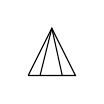
\begin{tikzpicture}[scale=0.6]
\draw (0,0) -- (0.5,1) -- (1,0) -- (0,0);
\draw (0.5,1) -- (0.25,0);
\draw (0.5,1) -- (0.72,0);
\end{tikzpicture}
\end{adjustbox}

$\mathfrak g$ ест. действует, $S$ порожд. ими и подобиями
[зачёркнуто: \Unclear{GELFAND-P000216}{cancelled-dilation}{растя...}]
сжатиями к вершине (и в точку).

\underline{Аксиомы.} $1^{\circ}$. $T$ стягиваемо преобразованиями из $S$ в отмеч. точку $\ast$.

$2^{\circ}$. $\mathfrak g$ замкн. в группе всех гомеом. $T$ в себя.

$3^{\circ}$. $\ast$ неподвижна отн. всех преобр. из $S$.

$4^{\circ}$. $\varphi_t:T\longrightarrow T$
\begin{equation*}
\begin{gathered}
\varphi_0=\text{тожд.},\quad\varphi_t\in S\quad\text{—}\\
\varphi_1(T)=\ast
\end{gathered}
\end{equation*}
— гомотопия аксиомы $1^{\circ}$.

Тогда сущ. $\varphi_t$, такие что
$\varphi_t$ при $t<1$ топологич. вложения.

$5^{\circ}$. $S$ содержит все преобр. $\mathfrak g$ и отображения,
близкие к отобр. $\mathfrak g$ в $S$, суть топ. вложения.

$U(1)\subset S$ сост. из вложений.

В этой ситуации опред. пр-ва
\begin{equation*}
\begin{adjustbox}{max width=\linewidth}
\begin{tikzcd}
\mathcal E_{\mathfrak g} \arrow[d] \\
S_{\mathfrak g}
\end{tikzcd}
\end{adjustbox}
\end{equation*}
, действие $\mathfrak g$ на $\mathcal E_{\mathfrak g}$ — универс. главное рассл.
\begin{equation*}
\underbrace{T\times\cdots\times T}_{I\text{ раз}}\qquad\text{тих. топология.}
\end{equation*}

$6^{\circ}$. $\mathfrak g$ действует эффективно на $T$,
(иначе \Unclear{GELFAND-P000216}{final-abbreviation}{удвл.} точка)

\SourcePage{GELFAND-P000217}{unlabelled}
Элемент \Unclear{GELFAND-P000217}{group-letter}{$\mathcal E_{\mathfrak g}$} — всякое вложение $T\subset T^I$, такое
что композиции его со всеми проекциями лежит в $S$.

1) $T=\mathbb R^n$ — все $n$-реперы.

2) $T=C\mathfrak g$, $\mathcal E_{\mathfrak g}=C\mathfrak g\times\ldots\times C\mathfrak g\setminus\{*,\ldots,*\}$.

$\mathfrak g$ действует в $\mathcal E_{\mathfrak g}$ домножением на преобр. из $\mathfrak g$.

\begin{equation*}
I\text{ конечно}\quad\Rightarrow\quad
\begin{aligned}
&1)\ \text{обычное классиф. пр-во}\\
&2)\ \text{констр. Милнора с не очень сущ. изменением.}
\end{aligned}
\end{equation*}

$\mathfrak g=\mathbb R$, $T={}$
\begin{adjustbox}{max width=\linewidth}
\begin{tikzpicture}[baseline=-0.5ex]
\draw (0,0)--(1.6,0);
\fill (0,0) circle (1.5pt);
\end{tikzpicture}
\end{adjustbox}
\qquad $\mathcal E_{\mathfrak g}$ — послед. неотр. чисел.

Для каждого $T$ своё опред. лок. тривиальности.

\begin{adjustbox}{max width=\linewidth}
\begin{tikzcd}[row sep=small]
E \arrow[d,"\mathfrak g"]\\ X
\end{tikzcd}
\end{adjustbox}
лок. трив., если индуц. рассл.
\begin{adjustbox}{max width=\linewidth}
\begin{tikzcd}[row sep=small]
E^{\#} \arrow[d,"T"]\\ X
\end{tikzcd}
\end{adjustbox}, облад. св-вом:

$\forall x\ \exists$ отобр. $E^{\#}\longrightarrow T$, гомеом. на слое над $x$ и
$\forall$ слое есть преобр. из $S$.

\underline{Теорема.}

Всякое расслоение отображается в это.

($X$ — все хаусдорфовы)

Определено $H^q_{\mathrm{alg}}(\mathfrak g;\mathbb R)$

\underline{Теорема.}

Каковы бы ни были $T$ и $S$ $H^q_{\mathrm{alg}}(\mathfrak g,\mathbb R)$
не зависит от их выбора

(Вместо $\mathbb R$ можно брать группу $A$)

\underline{Что будет?}

Успенский, Лекции по логике 2

Лидский, Асимптотика соб. ф-й (по Hörmander'у)

Синай, Условия на диффеом., при к-рых есть инвар. мера

Каждан, Дискр. группы — решение пробл. Сельберга

Кушниренко, Аналит. действие полупр. группы в окр. неподв. точки — линейно
% GELFAND-0023. Diplomatic transcription from the ten assigned original PNG frames.
% Review coordinates refer to original 2000 x 2456 source pixels, origin top left.
% Bounding boxes are (x0,y0,x1,y1), with right and bottom edges exclusive.
% Enlargement factors describe raster display only, not additional source detail.
% Source images remain authoritative. No external continuation has been supplied.
\SourcePage{GELFAND-P000218}{7}
% Full original frame inspected: bbox=(0,0,2000,2456).
% Review crop text-left: bbox=(120,0,640,445); enlargement=3x.
% Review crop text-right: bbox=(580,0,1240,440); enlargement=3x.
% Review crop interpolation-end: bbox=(815,245,950,300); enlargement=8x.
% Review crop power: bbox=(540,130,630,202); enlargement=8x.
Тюрина и С. Гельфанд\quad обзор работ Фама.

Аносов и Маслов

И. Бернштейн\quad $P^{\lambda}$

Гельфанд, Граев

С. Г. Крейн\quad \Unclear{GELFAND-P000218}{list-interpolation}{Интерполяции / Интерполяция}

$\begin{gathered}\text{Березин}\\\text{Кириллов}\end{gathered}$,\quad Грассманов анализ.

\begin{center}
$\text{—}\,\bullet\,\text{—}$
\end{center}

\SourcePage{GELFAND-P000219}{unlabelled}
% Full original frame inspected: bbox=(0,0,2000,2456).
% Review crop upper-left: bbox=(100,455,920,960); enlargement=2x.
% Review crop upper-right: bbox=(815,610,1860,975); enlargement=2x.
% Review crop middle: bbox=(105,940,1780,1375); enlargement=1x.
% Review crop lower: bbox=(25,1370,1950,2400); enlargement=1x.
% Review crop faded-top: bbox=(1390,735,1560,831); enlargement=6x.
% Review crop cancelled-date: bbox=(410,487,545,550); enlargement=8x.
% Review crop symmetric-word: bbox=(880,1220,1770,1315); enlargement=3x.
% Review crop dual-norm: bbox=(670,1960,1045,2130); enlargement=4x.
$16/\underline{\overline{\mathrm{X}}}$\quad \Unclear{GELFAND-P000219}{heading-cancelled}{[Зачёркнуто: неразборчиво.]}\quad \underline{С. Г. Крейн.}

\underline{Об интерполяции линейных операторов.}

\begin{equation*}
\left.
\begin{aligned}
 E_0,\ &\overset{A}{\longrightarrow}\ F_0,\\
 E_1,\ &\overset{A}{\longrightarrow}\ F_1,
\end{aligned}
\right\}\quad\text{банаховы пр-ва,}
\end{equation*}
\Unclear{GELFAND-P000219}{upper-embedding}{все вложенные / все вложены} в одно Т.Л.П. (левые и правые)

$A$ ограничен.

$E$, $F$ — интерпол. пара, если $\forall\ A$ из огранич.
при $0$ и $1$ следует огр. $A:E\longrightarrow F$.

Все пр-ва будут пр-вами суммир. функций.

Банахово пр-во сумм. ф-й [Вписано под строкой: на $[0,1]$.]
\Unclear{GELFAND-P000219}{definition-abbreviation}{на / наз.} симметрическим, если

1) $y(t)\in E$
\begin{equation*}
 |x(t)|\leq |y(t)|\quad\Longrightarrow\quad x\in E
 \qquad\text{и}\qquad \|x\|\leq\|y\|
\end{equation*}

2) Норма не меняется при преобр., сохр. меру
(можно рассм. равноизмеримую монотонную)

Тогда $L_\infty\subset E\subset L_1$.

\underline{Примеры.} 1)
\begin{equation*}
 \int_0^1 x^*(t)\,d\psi(t),\qquad \psi(t)\text{ — монот.}
 \qquad\text{— \underline{типа Лоренца}}
\end{equation*}
$x^*(t)$ — перестановка $|x(t)|$

2) Двойств.\quad
$\displaystyle\sup_e\frac{\int_e|x(t)|\,dt}{\psi(me)}$

3) и пр-ва Орлич (в них входят $L_p$)

[Слева над строкой:] 1-й шаг.

Теор. Рисса-Торина.

\SourcePage{GELFAND-P000220}{unlabelled}
% Full original frame inspected: bbox=(0,0,2000,2456).
% Review crop top: bbox=(115,0,1940,610); enlargement=1x.
% Review crop middle: bbox=(60,590,1950,1240); enlargement=1x.
% Review crop lower: bbox=(45,1200,1950,2456); enlargement=1x.
% Review crop names: bbox=(120,610,615,700); enlargement=3x.
% Review crop diagrams: bbox=(112,1440,785,1640); enlargement=3x.
% Review crop cancelled-space: bbox=(674,1360,881,1445); enlargement=6x.
% Review crop minimal-word: bbox=(1640,672,1925,759); enlargement=4x.
% Review crop limits: bbox=(120,2230,1360,2420); enlargement=2x.
% Review crop diagram-strokes: bbox=(590,1510,662,1593); enlargement=10x.
2-й шаг.

Теор. Марцинкевича.

(На концах треб. меньше)
\begin{equation*}
 n_x(\tau)=\operatorname{mes}\{t:|x(t)|\geq\tau\}
\end{equation*}
\begin{equation*}
 [n_{Ax}(\tau)]^{1/q_i}\leq\frac{C}{\tau}\|x\|_{L_{p_i}}
\end{equation*}
— менее огр. условие.

Большинство опер. анализа на концах удовл. усл. Марцинкевича

\underline{Мацаев и Дикарев} — точнее из $L_p$ в более узкое, чем $L_q$
пр-во (типа Лоренца)! — и оно уже минимально (посередине)

(Минимален для \underline{всех} операторов
в условиях как Марцинкевича и Рисса-Торина) —

— это для улучшающих операторов:
\begin{equation*}
\begin{gathered}q_1>p_1\\q_2>p_2\end{gathered}
\quad\Big\Vert\quad\text{— как и теор. Марцинкевича.}
\end{equation*}

$p=q$ — перев. в себя — тогда и все остальные шкалы тоже.

Пусть
$\begin{gathered}L_1\longrightarrow L_1\\L_\infty\longrightarrow L_\infty\end{gathered}$
\quad и $\|A\|\leq1$

Перечислить все \Unclear{GELFAND-P000220}{middle-cancelled}{[Зачёркнуто: неразборчиво.]} пр-ва, для к-рых тоже $\|A\|\leq1$.

\SourceFigure{GELFAND-P000220}{diagram-pair}{[Два рисунка: слева прямоугольник, справа ромб; в каждом оси со стрелками вправо и вверх. Подписи: «в себя», «в себя». Дополнительные наклонные штрихи у нижнего правого края требуют сверки с источником.]}

[Справа от рисунков:] лин. опер. (2-мерн. случай).

Док., что это все симметрические нормы и только они.

Общая теорема — Б. С. Митягин.

Необх. и дост., чтобы пр-во было симметрическим.

(и в $\infty$-мерн. случае)

$L_p\overset{A}{\longrightarrow}L_p$\qquad что тогда?

$p\ne1,\infty$

(случ. Марцинкевича)

\begin{equation*}
 \|\chi_e\|_E=\varphi(me).
\end{equation*}
[Под $\chi_e$ проведена черта к подписи:] хар. ф-я $e$.

(симметр. опять необходима)

получ. ф-я $\varphi(t)$ — хар-ка пр-ва $E$.
\begin{equation*}
 \ell_E=\underline{\lim}_{t\to0}\frac{\varphi(2t)}{\varphi(t)}
 \qquad
 u_E=\overline{\lim}_{t\to0}\frac{\varphi(2t)}{\varphi(t)}
 \qquad 1\leq\ell_E\leq u_E\leq2
\end{equation*}

\SourcePage{GELFAND-P000221}{9}
% Full original frame inspected: bbox=(0,0,2000,2456).
% Review crop top: bbox=(140,10,1965,580); enlargement=1x.
% Review crop middle: bbox=(130,540,1980,1340); enlargement=1x.
% Review crop lower: bbox=(100,1325,1970,2425); enlargement=1x.
% Review crop exponents: bbox=(300,385,830,575); enlargement=4x.
% Review crop hausdorff: bbox=(630,935,1285,1160); enlargement=3x.
% Review crop polya-name: bbox=(245,1040,590,1140); enlargement=4x.
% Review crop where-strokes: bbox=(1605,605,1830,705); enlargement=6x.
% Review crop gelfand-parenthesis: bbox=(1565,1435,1960,1525); enlargement=4x.
% Review crop same-letter: bbox=(405,2060,775,2165); enlargement=3x.
% Review crop coefficients: bbox=(1205,2205,1580,2407); enlargement=3x.
% Review crop square: bbox=(145,1782,270,1898); enlargement=5x.
Для $L_p$ они оба равны $2^{1/p}$

Огранич. всех таких $A$ в $E$ $\Longleftrightarrow$ $1<\ell_E\leq u_E<2$

(1-я теор. Семёнова)

Теор. Митягина не обобщена.
\begin{equation*}
 L_{1/\alpha}\longrightarrow L_{1/\alpha-\Delta}
\end{equation*}
\Unclear{GELFAND-P000221}{upper-target-exponent}{[Индекс справа: $1/\alpha-\Delta$ / $1/(\alpha-\Delta)$.]}

$0<\Delta\leq\alpha_0<\alpha<\alpha_1$.

Как перечислить пр-ва, в к-рых опер. такого типа огранич.?
\begin{equation*}
 2^{\alpha_0}<\ell_E\leq u_E<2^{\alpha_1}\quad\Longrightarrow\quad E\longrightarrow E_\Delta,
\end{equation*}
где \Unclear{GELFAND-P000221}{after-where-cancelled}{[После «где» два неразборчивых густых знака.]}
\begin{equation*}
 \|x\|_{E_\Delta}=\|x^*(t)t^{-\Delta}\|_E
\end{equation*}
(Это обобщ. теор. Дикарева и Мацаева — лучшее пр-во)

\underline{Прилож.:}\quad нер. Хаусдорфа-Юнга
\begin{equation*}
 \sqrt[p]{|c_k|^p}\leq\|x\|_{L_p}\qquad\text{— из теор. Рисса}
\end{equation*}
\Unclear{GELFAND-P000221}{hausdorff-formula}{[Запись под первым корнем сохранена; требует сверки.]}

нер-во Пойа:
\begin{equation*}
 \sqrt[p]{\sum k^{p-2}c_k^{*p}}\leq C\|x\|_{L_p}
\end{equation*}
$c_k^*$ — монот. перест. $|\ |$ коэфф.

Для монот. убыв. коэфф. Фурье — двустор. нер-ва (Харди-Литлвуд)

Между $L_1$ и $L_{1,5}$ нет гильб. интерпол. пр-ва (Семёнов)

\underline{Вопр. Гельфанда:} абстр. описание интерпол. пр-в.
(неизв., пр-ва ли они ф-й.)

\underline{Я. Синай.}

\underline{Построение инвар. мер гладких отобр.}\quad\underline{Марковские разб.}

\begin{adjustbox}{max width=\linewidth}
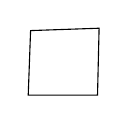
\begin{tikzpicture}
\draw (0,0)--(0.03,0.82)--(0.9,0.85)--(0.88,0)--cycle;
\end{tikzpicture}
\end{adjustbox}
\quad
$T(x_1,x_2)=(ax_1+bx_2,\ cx_1+dx_2)$ — отобр. тора

и $T_1$ — другое.

Когда сущ. измеримое отобр. тора, $M\overset{U}{\longrightarrow}M$,
что $UT_1=T_2U$.

\Unclear{GELFAND-P000221}{torus-map-indices}{[Обозначения $T$, $T_1$, $T_2$ сохранены.]}

Иррац. соб. знач. $\Rightarrow$ веществ. $\Rightarrow$ эргодично, спектр
счётнокр. лебеговский.

Энтропия $h(T)=\ln\lambda$\quad $(\lambda>1)$

\SourcePage{GELFAND-P000222}{unlabelled}
% Full original frame inspected: bbox=(0,0,2000,2456).
% Review crop top: bbox=(130,25,1980,450); enlargement=1x.
% Review crop matrix-region: bbox=(165,425,1970,1135); enlargement=1x.
% Review crop lower-middle: bbox=(130,1130,1980,1930); enlargement=1x.
% Review crop bottom: bbox=(155,1900,1960,2435); enlargement=1x.
% Review crop transition-entries: bbox=(250,455,1310,585); enlargement=3x.
% Review crop identity-example: bbox=(460,755,1980,909); enlargement=2x.
% Review crop cancellations: bbox=(307,1220,740,1408); enlargement=4x.
% Review crop example-cancelled: bbox=(1925,770,1978,835); enlargement=10x.
% Review crop eigenvector: bbox=(1430,1380,1945,1495); enlargement=4x.
% Review crop probabilities: bbox=(1190,1890,1518,2060); enlargement=5x.
% Review crop entropy-weights: bbox=(650,2110,1420,2245); enlargement=3x.
Если $h$ совп., то ещё не линейно сопряж. (есть другие-инв.)

Но метрически они подобны! ($U$ — разрывное, но измеримое)

$U$ — гомеом. $\Longrightarrow$ он линеен (можно док.)
(для любых комп. аб. групп)

$\Omega_\Pi$ — пр-во послед. $\omega=\{i_n\}$ — беск. в обе стороны послед.

$i_n\in\{1,\ldots,S\}$

\begin{equation*}
 \underset{\text{порядка }S}{\Pi}=\|x_{ij}\|,\quad x_{ij}=1,0
 \qquad \pi_{i_n i_{n+1}}=1
\end{equation*}
(только такие послед. $\omega$ допуст.)

\Unclear{GELFAND-P000222}{matrix-entry-notation}{[Буквы $x_{ij}$ и $\pi_{ij}$ сохранены.]}

Будем считать, что $\Pi^k$ — из полож. элем.

Рассм. сдвиг (преобр. сдвига на $\Omega$).

\underline{Пример.}\quad
$\begin{pmatrix}1&0\\0&1\end{pmatrix}$ — не уд. усл., но $\Omega$ — послед.
только из $1$ или \Unclear{GELFAND-P000222}{identity-example-cancelled}{[Зачёркнутый знак: неразборчиво.]} только из $2$

$\begin{pmatrix}1&1\\1&1\end{pmatrix}$ — всё можно ставить

$\begin{pmatrix}1&1\\1&0\end{pmatrix}$ — посмотреть.

на $\Omega_\Pi$ задать бы инв. меру $\mu$ с $\max$ энтропией:

\Unclear{GELFAND-P000222}{before-entropy-cancelled}{[Слева от формулы зачёркнутая неразборчивая запись.]}
\begin{equation*}
 h=\max_\mu h_\mu(T)
\end{equation*}
(\Unclear{GELFAND-P000222}{shift-parenthesis-cancelled}{[Зачёркнуто: где / сдв.]} $T$ — это сдвиг).

Надо рассмотреть $e$ с полож. коорд.\quad $\lambda e=\Pi^*e$, $\lambda>0$

(единств.)

\Unclear{GELFAND-P000222}{eigenvector-star}{[Звёздочка при $\Pi$ сохранена.]}

( Г. Если все элем. и все миноры 2-го порядка $>0$, то
сущ. 2 соб. вектора, 1-й с полож. элем., 2-й — с
1-й переменой знака —

— матр. миноров 2-го пор. — предст. самой матр. во внешнем произв.)

Рассм. цепь Маркова с вер. $\displaystyle p_{ij}=\frac{e_j\pi_{ij}}{\lambda e_i}$ —

[Справа:] — энтроп. — $\ln\lambda$

\begin{equation*}
\left[
\begin{gathered}
\text{Вообще энтр. цепи Маркова}\\
 h=\sum_i e_i\left(-\sum_j\ln p_{ij}\,p_{ij}\right)
\end{gathered}
\right.
\end{equation*}
\Unclear{GELFAND-P000222}{entropy-weights}{[Вес внешней суммы: $e_i$.]}

мера с $\max$ энтропией единственна.

Мера в $\Omega_\Pi$ на $\Sigma$-алг., порожд. цилиндрич. мн-вами.

\SourcePage{GELFAND-P000223}{10}
% Full original frame inspected: bbox=(0,0,2000,2456).
% Review crop top: bbox=(80,0,1985,730); enlargement=1x.
% Review crop central: bbox=(50,705,1900,1610); enlargement=1x.
% Review crop bottom: bbox=(85,1620,1910,2425); enlargement=1x.
% Review crop type-letters: bbox=(670,150,1465,447); enlargement=3x.
% Review crop hyperbolic-word: bbox=(1220,803,1470,902); enlargement=5x.
% Review crop bibliography: bbox=(137,1715,1770,1833); enlargement=2x.
% Review crop lower-cancellations: bbox=(127,1795,518,2027); enlargement=4x.
% Review crop integral-details: bbox=(645,1802,1640,2132); enlargement=3x.
% Review crop page-label: bbox=(1830,22,1955,96); enlargement=6x.
% Review crop leray-name: bbox=(370,1655,520,1740); enlargement=6x.
% Review crop small-cancelled: bbox=(392,1955,463,2030); enlargement=10x.
а) $\{a_1^1,\ldots,a_p^1;\ a_1^2,\ldots,a_q^2;\ b_1^1,\ldots,b_r^1;\ b_1^2,\ldots,b_s^2\}$

$\Pi$
\begin{equation*}
 \text{из }\left.\begin{gathered}\alpha^1\\\alpha^2\end{gathered}\right\}
 \longrightarrow\alpha^1\text{ или }B^1
\end{equation*}
\begin{equation*}
 \text{из }\left.\begin{gathered}\beta^1\\\beta^2\end{gathered}\right\}
 \longrightarrow\alpha^2\text{ или }B^2
\end{equation*}
\Unclear{GELFAND-P000223}{alphabet-type-letters}{[В переходах не вполне различимы $\alpha/a/A$ и $\beta/b/B$.]}

[На правом поле, за двойной вертикальной чертой:]
строится по целоч. матр. 2-го пор. разбиение.

$\lambda^2-(p+s)\lambda+(ps-qr)=0$,\qquad
\fbox{\fbox{$ps-qr=1$}}

[Под рамкой:] условие.

б) $\Omega_{\Pi_1}$\qquad $\pi_{ij}=1$ и $\pi_{N1}=0$ (только на 1-м месте)

\underline{Предл.}\quad\underline{Сдвиги в а) и б) изоморфны.}

[Слева выделено скобкой:]
Теперь всё свод. к док-ву того, что алгебр. автоморфизм $\Rightarrow$

$\Rightarrow$ разбиение.

Док-во предл.

Алфавит б): $A_1,\ldots,A_p$,\quad $B_1,\ldots,B_s$.

(Изоморфизм любых 2-х $\Omega_\Pi$ с одинаков. энтропией).

Кодируются разные группы (с пом. символов $A_i,B_i$).

Пр-во с 1-й $\max$ мерой перех. в пр-во с другой $\max$ мерой.

\underline{След. раз:} Марк. разбиения и как с их помощью строятся инв. меры.

$23/\underline{\overline{\mathrm{X}}}$.\quad \underline{Лерэ.}
\quad\underline{Особенности фейнмановских интегралов.}

N. Nilsson, Arkiv för Math. (Swede)\quad 1964–1965

(уч. Гординга)

\Incomplete{GELFAND-P000223}{lower-crossed-formula}{Зачёркнутая формульная запись под «(уч. Гординга)» не расшифрована: возможное начало $J(\ldots)$, остальные символы неразборчивы.}

\Unclear{GELFAND-P000223}{lower-crossed-symbol}{[Отдельный зачёркнутый знак: $J$ / $\gamma$.]}

\begin{equation*}
 J(t)=\int_{\gamma^q(t)}\omega(t,\xi)
\end{equation*}
[От $\gamma^q(t)$ проведён указатель к подписи:] цикл относит $W(t)$

[Под $\xi$ проведена черта к подписи:]
однор. степ. $0$

$=0$ на $W(t)$

$t\in T=C^n$,

$\xi\in C^{\ell+1}$

$\omega(t,\xi)$ на $P^\ell$, т.к. однородна; там и цикл.

\SourcePage{GELFAND-P000224}{unlabelled}
% Full original frame inspected: bbox=(0,0,2000,2456).
% Review crop top: bbox=(90,15,1970,540); enlargement=1x.
% Review crop upper-middle: bbox=(80,490,1980,1290); enlargement=1x.
% Review crop lower: bbox=(55,1300,1990,2440); enlargement=1x.
% Review crop discriminant: bbox=(220,150,1440,305); enlargement=3x.
% Review crop residue: bbox=(225,552,1385,877); enlargement=3x.
% Review crop theorem-side-note: bbox=(1470,1025,1880,1110); enlargement=5x.
% Review crop manifolds: bbox=(210,1860,601,2125); enlargement=4x.
% Review crop intersection-sign: bbox=(770,288,849,471); enlargement=7x.
% Review crop cycle-argument: bbox=(395,812,572,886); enlargement=8x.
% Review crop growth-exponent: bbox=(824,1550,1074,1643); enlargement=6x.
$W(t)=\bigcup_k W_k(t)$ — гиперплоск., алгебр. ф-и $t$,
могут быть особенности (не в общем положении)

$t\in S_0[W]\Longleftrightarrow$ в ней измен. размерность пересеч. любого числа.

Def:
\begin{equation*}
 \gamma^{q-m}(t)=\bigcap_{j=1}^m V_j(t),\qquad V_j(t)=v_j(t,x)=0
\end{equation*}
\Unclear{GELFAND-P000224}{intersection-sign}{[Крупный знак: $\bigcap$ / $\bigwedge$.]}

[Под $v_j(t,x)=0$ черта к подписи:] алгебр. мн-ие

Надо предпол.
\begin{equation*}
 \frac{\omega(t,\xi)}{[v_1(t,\xi)]^{1+\beta_1}\ldots[v_m]^{1+\beta_m}}
 \qquad\text{— опред. на }P
\end{equation*}

[Слева:] Вычет
\begin{equation*}
 J(t)=\int_{\gamma^{q-m}(\xi)}
 \frac{d^{\beta_1+\ldots+\beta_m}\omega}
 {[dv_1]^{1+\beta_1}\wedge\ldots\wedge[dv_m]^{1+\beta_m}}
\end{equation*}
\Unclear{GELFAND-P000224}{residue-cycle-argument}{[Аргумент под интегралом: $\xi$ / $s$.]}

Особ. носитель в общ. случае тоже описывается

(На накрыв. пр-ве дополнения форма будет голоморфна)

\underline{Теор.} Тогда $J(t)$ имеет алгебр. син. носитель.

\Unclear{GELFAND-P000224}{theorem-margin-note}{[Приписка справа: типа ст. алгебр. / типа см. алгебр.]}

(т.е. в $T$ сущ. алг. мн-ие, что $J(t)$ голом. на накр. дополн.)

Лерэ описал син. носит. в случае плоскостей.

$30/\underline{\overline{\mathrm{X}}}$\quad\underline{Синай.}

\underline{$U$-диффеом:}\quad хар. $\exp$ рост расст. между близкими точками
(разбегание)

либо при $t\longrightarrow+\infty$, либо при $t\longrightarrow-\infty$.
\begin{equation*}
 \frac{d(T^n x,T^n y)}{d(x,y)}\geq ae^{cn}
 \qquad\begin{gathered}n>0\\\text{или }n<0\end{gathered}
 \qquad(x,y\text{ — близки})
\end{equation*}
\Unclear{GELFAND-P000224}{growth-negative-time}{[Показатель первой экспоненты: $cn$.]}

Рассм. точки $d(T^n y,T^n x)\leq ae^{-cn}d(y,x)$,

Пусть $\forall\ x$ это $k$-мерное подмн-ие.

\begin{adjustbox}{max width=\linewidth}
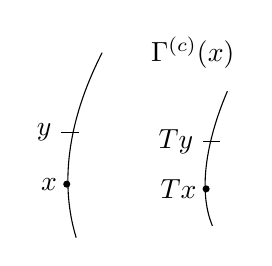
\begin{tikzpicture}
\draw (0.15,0) .. controls (-0.05,0.65) and (0.02,1.45) .. (0.48,2.35);
\fill (0.03,0.68) circle (0.045);
\node[left] at (0.03,0.68) {$x$};
\draw (-0.04,1.34)--(0.19,1.34);
\node[left] at (-0.04,1.34) {$y$};
\draw (1.88,0.15) .. controls (1.68,0.63) and (1.83,1.3) .. (2.07,1.86);
\fill (1.8,0.62) circle (0.045);
\node[left] at (1.8,0.62) {$Tx$};
\draw (1.76,1.22)--(1.98,1.22);
\node[left] at (1.76,1.22) {$Ty$};
\node at (1.63,2.35) {$\Gamma^{(c)}(x)$};
\end{tikzpicture}
\end{adjustbox}

Это сжимающееся подмн-ие (отсюда индекс \underline{$c$})
\begin{equation*}
 d(T^n y',T^n x)\leq ae^{+cn}d(y',x)
 \qquad(n\longrightarrow-\infty).
\end{equation*}

Получим подобн. $\Gamma^{(p)}(x)$ — расшир. подмн-ие.

($\ell$-мерное).

Тогда выбор не зав. от $a$ и $c$.

\SourcePage{GELFAND-P000225}{11}
% Full original frame inspected: bbox=(0,0,2000,2456).
% Review crop top: bbox=(120,5,1970,740); enlargement=1x.
% Review crop middle: bbox=(100,698,1990,1475); enlargement=1x.
% Review crop bottom: bbox=(110,1430,1997,2205); enlargement=1x.
% Review crop foliations: bbox=(162,270,1265,365); enlargement=3x.
% Review crop lattice-diagram: bbox=(275,447,552,682); enlargement=4x.
% Review crop group-notation: bbox=(185,765,630,957); enlargement=4x.
% Review crop eigenvalue-crossing: bbox=(1140,1290,1985,1390); enlargement=3x.
% Review crop right-bottom-note: bbox=(1810,2045,1999,2190); enlargement=5x.
% Review crop cancelled-before-eigenvalues: bbox=(1165,1294,1334,1374); enlargement=8x.
% Review crop terminal-arrow: bbox=(1913,1290,1999,1385); enlargement=8x.
% Review crop nilpotence-parenthesis: bbox=(150,1444,1160,1550); enlargement=3x.
$U$-система:
$k+\ell=n$ и кас. пр-ва к подмн. равном. трансверсальны

1. $k+\ell=n$

2. трансверс.

3. Гладкость (не выпис. явно).

Получаем 2 слоения $\gamma^{(\mathrm{c})}$ и $\gamma^{(\mathrm{p})}$.

\underline{Пример:} лин. преобр. тора
$(x,y)\longrightarrow(ax+by,cx+dy)$.
\begin{equation*}
 \begin{vmatrix}a&b\\c&d\end{vmatrix}=1.
\end{equation*}
\SourceFigure{GELFAND-P000225}{lattice-diagram}{[Рисунок: две пересекающиеся семьи наклонных параллельных линий; оси со стрелками вверх и вправо. Точное число линий и их соединения в густых пересечениях не установлены.]}

(паралл. соб. напр.).

Нелин. возмущение (периодич. и гладкое) — тоже
$U$-диффеом. и число вращ. то же.

\underline{Метод постр. $U$-дифф.}

\Unclear{GELFAND-P000225}{group-notation}{$\mathfrak{G}$ / $g$} — гр. Ли, $\Gamma$ — дискр. подгр.

$\mathfrak{G}/\Gamma$ — компактна.

$T_{\mathrm{alg}}$ — алг. автом. $\mathfrak{G}$, ост. неподв. $\Gamma$
\quad$(T_{\mathrm{alg}}\Gamma=\Gamma)$

[Под $T_{\mathrm{alg}}$, соединено дугой:] автом. как группы

Тогда он действ. на $\mathfrak{G}/\Gamma$.

Рассм. $G$ — алгебру Ли; $\hat T_{\mathrm{alg}}$ — соотв. автом. $G$; если его

[У левого края следующей строки:] соб. знач.

Среди них нет \Unclear{GELFAND-P000225}{cancelled-before-eigenvalues}{[Зачёркнуто: $\Longleftrightarrow$ / $\Longrightarrow$.]} соб. знач. $=1$ по $\operatorname{mod}$ \Unclear{GELFAND-P000225}{terminal-arrow}{[Знак после mod: $\Leftrightarrow$ / зачёркнутый знак.]}

$\Longleftrightarrow$ это $U$-диффеом.

(\Unclear{GELFAND-P000225}{nilpotence-parenthesis}{Существуют / Существует} $\Longleftrightarrow G$ нильпотентна).

Дальше. Малое нелин. возмущение $T=T_{\mathrm{alg}}+\Delta T$ — тоже
$U$-дифф.
\underline{Осн. проблема:} топ. подобность алгебраич.

Для малых возмущ. — из общей теор. Аносова

(Малое возм. $U$-дифф. топ. подобно исходному).

Всегда.
\begin{equation*}
 M=M_1\cup M_2
\end{equation*}
$M_2$ — блужд. точки

$M_1$ — неблужд. точки. — на них вып. условие $U$

[На правом поле, отделено вертикальной чертой:] тоже гипотеза

\SourcePage{GELFAND-P000226}{unlabelled}
% Full original frame inspected: bbox=(0,0,2000,2456).
% Review crop top: bbox=(150,0,1998,725); enlargement=1x.
% Review crop middle: bbox=(150,690,1985,1500); enlargement=1x.
% Review crop bottom: bbox=(150,1450,1995,2456); enlargement=1x.
% Review crop holonomy-diagram: bbox=(180,95,590,310); enlargement=3x.
% Review crop holonomy-description: bbox=(706,114,1910,259); enlargement=3x.
% Review crop parallelogram-diagram: bbox=(730,415,940,560); enlargement=5x.
% Review crop boundary-diagram: bbox=(1330,1020,1570,1250); enlargement=5x.
% Review crop bottom-diagrams: bbox=(326,1717,694,2022); enlargement=4x.
% Review crop contracted-disk-text: bbox=(220,220,726,315); enlargement=3x.
% Review crop holonomy-symbol: bbox=(250,305,341,388); enlargement=8x.
% Review crop canonical-isomorphism: bbox=(1140,240,1622,318); enlargement=3x.
% Review crop union-symbol: bbox=(970,625,1052,700); enlargement=8x.
% Review crop theorem: bbox=(745,1665,1990,2008); enlargement=2x.
% Review crop theorem-alpha-gloss: bbox=(865,1840,1018,1959); enlargement=5x.
% Review crop final-formula: bbox=(837,2274,1640,2406); enlargement=3x.
Важное построение:

\begin{center}
\begin{adjustbox}{max width=\linewidth}
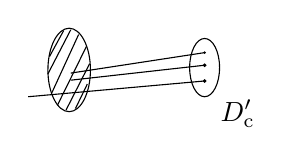
\begin{tikzpicture}[x=1cm,y=1cm]
 \draw (0,0) ellipse (0.27 and 0.53);
 \draw (-0.22,-0.29)--(0.12,0.45);
 \draw (-0.27,-0.05)--(0.02,0.51);
 \draw (-0.25,0.17)--(-0.07,0.50);
 \draw (-0.15,-0.45)--(0.22,0.30);
 \draw (-0.04,-0.51)--(0.26,0.08);
 \draw (0.08,-0.49)--(0.23,-0.18);
 \draw (1.72,0.03) ellipse (0.19 and 0.37);
 \draw (0.02,-0.04)--(1.72,0.22);
 \draw (0.02,-0.13)--(1.72,0.06);
 \draw (-0.52,-0.34)--(1.72,-0.14);
 \fill (1.72,0.22) circle (0.018);
 \fill (1.72,0.06) circle (0.025);
 \fill (1.72,-0.14) circle (0.025);
 \node[below right] at (1.80,-0.26) {$D'_{\mathrm{c}}$};
\end{tikzpicture}
\end{adjustbox}
\end{center}
Естеств. изом. наших кусочков. сжим. слоёв
(по несжим. слоям).

$D_{\mathrm{c}}$ — сжим. подмн. $\dim=k$.
\quad($\pi$ — канон. изом.)

$\pi$ не всегда гладко (!), но оно абс. непр., т. е. естеств.
меры перев. друг. в друга.

Параллелограмм: \SourceFigure{GELFAND-P000226}{parallelogram-diagram}{[Рисунок параллелограмма из отрезков слоений: две почти вертикальные кривые и несколько поперечных кривых; средние пересечения и число внутренних отрезков неразличимы.]} из отрезков слоений

(все принадл. ему слои кан. изоморфны: и сжим. и расшир.)
\begin{equation*}
 \Gamma(U)=\Gamma_{\mathrm{p}}(U)\cup\Gamma_{\mathrm{c}}(U)
\end{equation*}
Пусть есть система паралл. $U_i$, примык. друг к другу.
\begin{equation*}
 \begin{gathered}
 M=\bigcup\overline{U}_i\\
 U_i\cap U_j\subset\Gamma(U_i)\cap\Gamma(U_j)
 \end{gathered}
 \qquad(\Gamma\text{ — границы}).
\end{equation*}
$\alpha$ — такое разб. на пар-мы. Рассм. границы:
\begin{equation*}
 \begin{gathered}
 \Gamma_{\mathrm{p}}(\alpha)=\bigcup_i\Gamma_{\mathrm{p}}(U_i)\\
 \Gamma_{\mathrm{c}}(\alpha)=\bigcup_i\Gamma_{\mathrm{c}}(U_i)
 \end{gathered}
\end{equation*}
[Справа рисунок:]
\begin{center}
\begin{adjustbox}{max width=\linewidth}
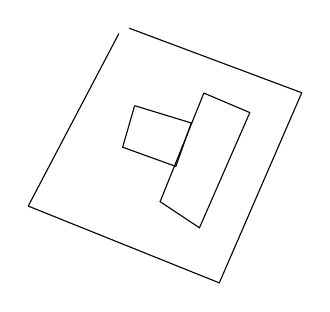
\begin{tikzpicture}[x=0.004cm,y=-0.004cm]
 \draw (121,710)--(409,162);
 \draw (442,145)--(990,350)--(728,954)--(121,710);
 \draw (679,351)--(825,413)--(665,779)--(540,696)--(679,351);
 \draw (459,391)--(639,446)--(590,584)--(421,523)--(459,391);
\end{tikzpicture}
\end{adjustbox}
\end{center}
Это $\alpha$ наз. марковским, если сущ. $m$, такое что
\begin{equation*}
 \fbox{$\begin{gathered}
 \Gamma_{\mathrm{p}}(T^{-m}\alpha)\subset\Gamma_{\mathrm{p}}(\alpha)\\
 \Gamma_{\mathrm{c}}(T^{+m}\alpha)\subset\Gamma_{\mathrm{c}}(\alpha)
 \end{gathered}$}
\end{equation*}
[Справа в рамке со ступенчатым левым краем:]

\underline{Теор.} (технич.) Марк. разб. сущ. и их
много: $\forall\alpha$, $\forall\varepsilon>0$ $\exists m$ и разб. $\widetilde\alpha$, что
оно будет отст. от исходного меньше чем на $\varepsilon$.

[Под $\alpha$ выносная подпись:] разб. на пар-мы

[Слева:] \SourceFigure{GELFAND-P000226}{bottom-diagrams}{[Слева отдельный наклонный четырёхугольник. Справа длинная узкая полоса снизу слева вверх вправо пересекает поперечные четырёхугольники у концов; точные соединения нескольких наложенных контуров у верхнего правого конца требуют сверки с оригиналом.]}

концы не могут быть в середине.

(исх. пар.)

\begin{center}$\text{—}\,\bullet\,\text{—}$\end{center}

Если $\alpha$ — разб. с $m$, то можно сделать $m=1$,
взяв пересечение
\begin{equation*}
 \alpha_1=\alpha\cdot T^{-1}\alpha\cdots\cdot T^{-m+1}\alpha\;\text{—}
\end{equation*}
— марковское с $m=1$

\SourcePage{GELFAND-P000227}{12}
% Full original frame inspected: bbox=(0,0,2000,2456).
% Review crop top: bbox=(150,0,1985,732); enlargement=1x.
% Review crop upper-middle: bbox=(125,687,1985,1320); enlargement=1x.
% Review crop lower-middle: bbox=(115,1290,1990,1855); enlargement=1x.
% Review crop bottom: bbox=(125,1850,1998,2456); enlargement=1x.
% Review crop mapping-symbol: bbox=(826,788,922,893); enlargement=8x.
% Review crop nonempty-note: bbox=(179,740,1739,808); enlargement=3x.
% Review crop nonunique-note: bbox=(1490,789,1930,870); enlargement=3x.
% Review crop overwritten-negation: bbox=(438,886,623,955); enlargement=6x.
% Review crop invariant-measure-diagram: bbox=(136,1330,387,1550); enlargement=4x.
% Review crop cancelled-group-word: bbox=(418,1670,659,1790); enlargement=4x.
% Review crop cancelled-before-chain: bbox=(1245,1786,1337,1865); enlargement=8x.
% Review crop bottom-matrix-indices: bbox=(936,1950,1827,2078); enlargement=4x.
% Review crop bottom-cancelled-word: bbox=(1201,2201,1690,2302); enlargement=4x.
% Review crop bottom-note: bbox=(1330,2296,1986,2414); enlargement=3x.
% Review crop final-diagrams: bbox=(133,1980,792,2305); enlargement=3x.
% Review crop heading-assumption: bbox=(1624,123,1962,287); enlargement=3x.
% Review crop first-sum-prime: bbox=(1218,1937,1386,2090); enlargement=6x.
% Review crop our-parallelograms: bbox=(1000,2225,1300,2306); enlargement=4x.
% Review crop measure-arrowheads: bbox=(193,1400,311,1502); enlargement=8x.
— из
\begin{equation*}
 \Gamma_{\mathrm{p}}(\alpha_1)=\Gamma_{\mathrm{p}}(\alpha)
 \cup\Gamma_{\mathrm{p}}(T^{-1}\alpha)\cup\cdots
 \cup\Gamma_{\mathrm{p}}(T^{-m+1}\alpha)
\end{equation*}
\underline{Символическая динамика для $U$-диффеом.}

(Пусть есть марк. разб. и с $m=1$)
\begin{equation*}
 \pi_{j_1j_2}=\begin{cases}
 1&V_{j_1}\cap TV_{j_2}\ne\varnothing\\
 0&\text{в ост. случаях}
 \end{cases}
\end{equation*}
$\Pi$

$\Omega_\Pi$ — пр-во из точек
\begin{equation*}
 \begin{gathered}
 \omega=\{\ldots\ j_{-n},\ldots,j_0,\ldots,j_n,\ldots\}\\
 \pi_{j_nj_{n+1}}=1.
 \end{gathered}
\end{equation*}
Сопоставим теперь
\begin{equation*}
 \omega\longrightarrow\bigcap_{-\infty}^{+\infty}T^n\overline{V}_{j_n}
 =x\in M\qquad(!)
\end{equation*}
(непусто из марковости и при мелком разб. из 1-й точки)

Получ. отображение $\varphi:\Omega_\Pi\longrightarrow M$

[Справа начата скобка:] (из неединств.

оно не \Unclear{GELFAND-P000227}{overwritten-negation}{[Зачёркнуто после «не»: возможно «вз.»; чтение не установлено.]} вз.-одн. из-за точек — границ пар-мов).

На мн-ве 2-й катег. вз.-однозначно.

\underline{Условие:} $\Pi^K$ из полож. элем. при нек-ром $K$.

(т. е. все слои $\Gamma^{(\mathrm{c})}$ и $\Gamma^{(\mathrm{p})}$ плотны на $M$ — это
необх. и достат.)

\underline{На каждом слое $\Gamma^{(\mathrm{c})}$ вводится $\sigma$-конечная мера $\lambda_{\mathrm{c}}$,}

причем

[Слева:] \SourceFigure{GELFAND-P000227}{invariant-measure-diagram}{[Рисунок: две изогнутые линии с подписями $A$ и $\widetilde A$; между ними несколько кривых слева направо с уклоном вниз. Число наложенных нижних кривых и наличие стрелок на всех их правых концах не установлены.]}

1) $\lambda_{\mathrm{c}}(A)=\lambda_{\mathrm{c}}(\widetilde A)$

(меры кан. изом. мн-в равны)

2) $\lambda_{\mathrm{c}}(TA)=h\lambda_{\mathrm{c}}(A)$
\quad$(h<1)$

($h$ — алгебр. число).

— доп. информ.

(Отраж. однор. структуры)

(В алг. \Unclear{GELFAND-P000227}{cancelled-group-word}{[Зачёркнуто: возможно «случае». Вписано сверху: $U$-автом.]} всё индуц. мерой Хаара.)

\underline{Следствие:} есть инвар. мера, $T$ явл. \Unclear{GELFAND-P000227}{cancelled-before-chain}{[Зачёркнуто: «б» / «в».]} конечн. цепью Маркова.

\underline{Построение этой меры:} $(n=2)$

\SourceFigure{GELFAND-P000227}{final-diagrams}{[Два рисунка. Слева область $V_i$ с криволинейными краями и выносной подписью: внутренние кривые, две поперечные отметки на средней кривой, стрелкообразные концы вниз влево и вверх вправо. Справа длинная изогнутая полоса пересечена двумя поперечными четырёхугольниками; на средней линии виден направленный вверх штрих. Точное сопряжение толстых линий внизу правой схемы и все направления концов требуют просмотра оригинала.]}

\begin{equation*}
 \lambda_i h^{-1}=\sum\lambda_i'=\sum\pi_{ii'}\lambda_{i'},\quad\text{т. е.}
\end{equation*}
\Unclear{GELFAND-P000227}{first-sum-prime}{[В первой сумме положение штриха допускает $\sum\lambda_i'$ / $\sum\lambda_{i'}$; сохранён его верхний уровень.]}
\begin{equation*}
 \fbox{$h^{-1}\vec\lambda=\Pi\vec\lambda$.}
\end{equation*}
— собств. вектор.

(Это при наших \Unclear{GELFAND-P000227}{bottom-cancelled-word}{[Зачёркнуто: неразборчиво.]} пар-мах).

На отрезке знач. меры есть. Далее из 2-го св-ва.

[Под последней строкой:] (на отр. поменьше)
\SourcePage{GELFAND-P000228}{unlabelled}
\Unclear{GELFAND-P000228}{title-ending}{Энтропия / Энтропии}
\Unclear{GELFAND-P000228}{matrix-dot}{$T=\left|\begin{array}{ccc}a&\cdot&b\\c&&d\end{array}\right|$}
$h(T)=\ln\lambda\quad(\lambda>1)$

\Unclear{GELFAND-P000228}{entropy-second-line}{$h(T)=\lambda$}
$\Rightarrow$ преобр. метрически изоморфны.

$\Omega_{\Pi_1}$ отобр. на $\Omega_{\Pi_0}$ (станд.) —
\Unclear{GELFAND-P000228}{earlier-abbreviation}{прежн. раз.}

И осталось тор. отобр. на $\Omega_{\Pi_1}$.

$\Pi_1$ определённого типа: 4 группы букв и св-ва
перех. — см. ранее.

\SourceFigure{GELFAND-P000228}{torus-partition}{Почти прямоугольная рамка с диагональными отрезками внутри; наклонные рёбра выходят за рамку вверх, вправо и вниз. Внутри сверху слева и снизу, а также в нижней выступающей части видна штриховка. Подписей вершин нет. Соединения наложенных линий не во всех местах различимы.}
— разб. тора на 2 параллелограмма
(стороны $\parallel$ соб. напр.)

Стороны леж. на прямой, прох. через 0
по собств. напр. (и \Unclear{GELFAND-P000228}{parenthetical-direction}{продолж.}).

Это Марковское разбиение (самое крупное).
Из-за него и удаётся решить пробл. изоморфизма.

\Unclear{GELFAND-P000228}{intersection-subscript}{$\bigcap T^nV_{\omega_n}$}
может сост. из больш. числа точек.

Рассм. сначала 4 пар-на:
\begin{gather*}
V_1\cap TV_1
\end{gather*}
\Unclear{GELFAND-P000228}{second-pair}{$V_2\cap TV_2$ / $V_2\cap TV_1$}
\begin{gather*}
V_1\cap TV_2
\end{gather*}
\Unclear{GELFAND-P000228}{fourth-pair}{$V_1\cap TV_2$}

(\Unclear{GELFAND-P000228}{uzhe-cancellation}{Уже (возможно зачёркнуто)} несвязн. разбиение. Образ. разбиение —
— его связные комп. Их числа соотв. —
— \Unclear{GELFAND-P000228}{component-counts}{$p,q,r,s$})

\SourcePage{GELFAND-P000229}{unlabelled}
\underline{1968 год.}

12/II \quad \underline{Вопрос} (Гельфанд)

$R$ — счётнонорм. кольцо:
\Unclear{GELFAND-P000229}{norm-final-index}{$\lVert xy\rVert_i\leq\lVert x\rVert_k\lVert y\rVert_\ell$}

\fbox{Теор. Гельфанд–Наймарк}
для \Unclear{GELFAND-P000229}{superscribed-mark}{неразборчивый надстрочный знак}
норм. кольц:
\Unclear{GELFAND-P000229}{ideal-space-notation}{$f(x^*x)\geq0\Rightarrow f(x)=\int_{\mathcal{M}_0}x(M)\,d\sigma(M)$}

\Unclear{GELFAND-P000229}{ideal-space-notation}{($\mathcal{M}_0$ — симм. ид.)}

Перенос — ? (Не всегда: надо
охар. аксиом. класс).

$x^*(M)=\overline{x(M')},\quad M=M'$ — симм.

$L^1$ со свёрткой, $\overline{x(-t)}=x^*(t)$
$\Rightarrow$ теор. Бохнера
\Unclear{GELFAND-P000229}{bochner-integral}{$\int_{-\infty}^{+\infty}e^{it\lambda}\,d\sigma(t)$}

\underline{И. Бернштейн.}\quad \underline{Топология Гротендика.}

$T$ — это след. совокупность:

1) Категория $\operatorname{Cat}T$ выделена (объекты — откр. мн-ва).

2) Выделены нек-рые сем-ва $\{\alpha_i:U_i\to U\}$,
называемые покрытиями

3) Выд. система, уд. аксиомам:

1. Сущ. пересечение — \underline{произведение} (расслоенное).

\begin{adjustbox}{max width=\linewidth}
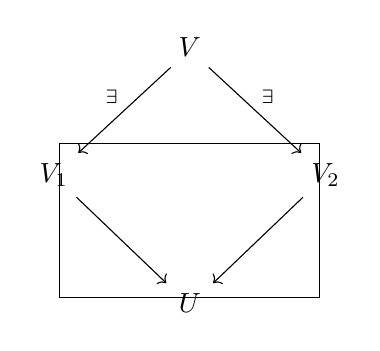
\begin{tikzpicture}
\node[inner sep=0] at (0,0) {
\begin{adjustbox}{max width=\linewidth}
\begin{tikzcd}[row sep=1.1cm,column sep=1.1cm]
& V \arrow[dl,"\exists"'] \arrow[dr,"\exists"] & \\
V_1 \arrow[dr] && V_2 \arrow[dl] \\
& U &
\end{tikzcd}
\end{adjustbox}};
\draw (-1.65,0.4) rectangle (1.65,-1.55);
\end{tikzpicture}
\end{adjustbox}
(коммут.).

— \underline{дано 3 об. и 2 отобр.}

\fbox{$V=V_1\times_U V_2$} — обозначение.
Тогда сущ.

\begin{adjustbox}{max width=\linewidth}
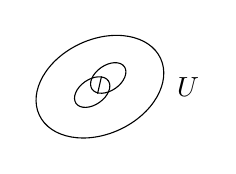
\begin{tikzpicture}
\draw[rotate=25] (0,0) ellipse (0.85cm and 0.6cm);
\draw[rotate=35] (-0.12,0) ellipse (0.25cm and 0.16cm);
\draw[rotate=35] (0.15,0.03) ellipse (0.25cm and 0.16cm);
\draw (-0.03,-0.09) -- (0.02,0.13);
\node at (1.12,0) {$U$};
\end{tikzpicture}
\end{adjustbox}

Треб. вып. универс. св-ва:

$\forall X$, и $\forall$
\SourceFigure{GELFAND-P000229}{universal-diagram}{Слева $X$, справа $V$, между ними сверху $V_1$ и снизу $V_2$. Различимы стрелки $X\to V_1$, $X\to V_2$, $V\to V_1$, $V\to V_2$. Соединение между $X$ и $V$ обведено, слева и справа имеются похожие на наконечники штрихи; направление этой стрелки не установлено. От середины соединения идёт выносная линия к подписи ниже справа.}
сущ. и единств.

От $U$ существенно зависит (в топ. Гротенд.)

(Если $V$ сущ., то он опред. однозн. по св-вам категории)

\SourcePage{GELFAND-P000230}{unlabelled}
\Unclear{GELFAND-P000230}{upper-right-label}{18 / 98}

2. $\{U\overset{id}{\longrightarrow}U\}$ — покрытие.

3. $\{V_i\to V\}$ — покр.

$\{V_{ij}\to V_i\}$ — покр.

$\Rightarrow\{V_{ij}\to V\}$ — покр.

4. $\{U_i\to U\}$ — покрытие

$\{V\to U\}$ — морфизм

Тогда $\{U_i\times_U V\to V\}$

\underline{Пример:} неразветвл. топология.

$X$ — обычн. топ. пр-во.

Откр. мн-во: $U\to X$ — лок. гомеоморфизм

($U$ — топ. пр.)

(накрытие над $X$ или его откр. \Unclear{GELFAND-P000230}{open-subset-word}{подмн-вом}).

Отображение
\begin{adjustbox}{max width=\linewidth}
\begin{tikzcd}
U \arrow[r] & X \\
V \arrow[u] \arrow[ur] &
\end{tikzcd}
\end{adjustbox}
(любое непр. с комм. диагр.)

$\{U_i\to U\}$ — покр., если образы
\Incomplete{GELFAND-P000230}{crossed-word}{Зачёркнутое слово не читается.}
покрывают.

\underline{Аксиома 1.}

\begin{adjustbox}{max width=\linewidth}

\begin{tikzpicture}
\draw[rotate=20] (0,0) ellipse (0.43cm and 0.35cm);
\end{tikzpicture}
\end{adjustbox}
$U$ — окр., $U$ — тоже окр., отобр. со степ. 2
$U\to U$.

\Unclear{GELFAND-P000230}{degree-two-product}{$U\times_U U=U$}.

\begin{adjustbox}{max width=\linewidth}
\begin{tikzcd}[row sep=small,column sep=small]
& U \arrow[dl] \arrow[dr] & \\
U \arrow[dr] && U \arrow[dl] \\
& U &
\end{tikzcd}
\end{adjustbox}

$U_1\times_X U_2$ —
\Unclear{GELFAND-P000230}{join-operations}{перемн. и склеив.}
— несвязное объед.

2 и 3 листа $\Rightarrow$ 6 листов

\begin{gather*}
\mathbb{Z}_2\times\mathbb{Z}_2\neq\mathbb{Z}_4,\\
\mathbb{Z}_2\times\mathbb{Z}_3=\mathbb{Z}_6.
\end{gather*}

\SourcePage{GELFAND-P000231}{unlabelled}
Предпучок: $\bullet$ функтор
\begin{gather*}
\operatorname{Cat}T\to\mathrm{Ab}\qquad\text{(контравар.)}\\
u\to P(u)\qquad v\to u\;\Rightarrow\;P(u)\to P(v)
\end{gather*}
Пучок — предпучок, удовл. аксиомам:

1. $\xi\in P(u)$

$\{u_i\to u\}$ — покрытие
\begin{equation*}
\xi\to\xi_i\qquad P(u)\to P(u_i)
\end{equation*}
$\xi$ — однозн. опр. $\xi_i$

2. и действ. опр., если $\xi_i$ совп. на пересеч. $u_i\times_u u_j$.

Когомологии Чеха определим
\begin{align*}
C^0&=P(u)\\
C^1&=\prod P(u_i)\\
C^2&=\prod P(u_i\times_u u_j).\\
C^3&=\prod P(u_i\times_u u_j\times_u u_k)
\end{align*}
$d$ опред. естеств

$\mathcal F\to\Gamma(X,\mathcal F)$ — функтор.

\Unclear{GELFAND-P000231}{gamma-gloss}{($\Gamma$ — аб. группа —\newline — пучок групп)}
\begin{equation*}
0\to\mathcal F_1\to\mathcal F_2\to\mathcal F_3\to0.
\end{equation*}
— \underline{точн. посл. пучков.}
\begin{equation*}
0\to\Gamma(\mathcal F_1)\to\Gamma(\mathcal F_2)\to\Gamma(\mathcal F_3)
\end{equation*}
(точный слева).

Сущ. производные функторы. $R^i:S\to\mathrm{Ab}$

$S$ — произв. пучки (категория).
\begin{equation*}
\to R^1(\mathcal F_1)\to\ldots\to R^2(\mathcal F_2)
\end{equation*}
($R^i$ — опр. однозначно).
\begin{equation*}
R^i(\mathcal F)\underset{\mathrm{def}}{=}H^i(X,\mathcal F).
\end{equation*}
\underline{Кон. группа.} Топ. Гротендика из представлений.

[Внизу справа: жёлтый значок речевого облачка с тремя чёрными горизонтальными линиями; верхние две длиннее нижней.]

\SourcePage{GELFAND-P000232}{unlabelled}
11/III \underline{Гельфанд} (и Кириллов)

$\mathfrak g$ — полупростая алгебра Ли, (над $C$)

$U(\mathfrak g)$ — её обёрт. алгебра

(полин. от обр. $e_1,\ldots,e_n$;
$e_i e_k-e_k e_i=\sum C^j_{ik}e_j$

$Z(\mathfrak g)$ — центр обёрт. алгебры

(её элем. — опер. Лапласа или Казимира).

Предст. $G\Rightarrow$ дифф. опер. и коммут.

[Справа:] $Z(\mathfrak g)$ — коммут. с действ. \Unclear{GELFAND-P000232}{centre-end}{групп}

Такое предст. обёрт. алг. дифф. операторами не обяз. точное.

На самой $G$ — точное (преобр.)

Для $Z(\mathfrak g)$ всё равно левые или правые.

$\mathfrak g$ — полупростая алгебра Ли. (над $C$).

$N_-$ — $\max$ нильпот. \Unclear{GELFAND-P000232}{nilpotent-corrections}{[зачёркнуто: группа алгебра]} [ниже вписано: группа] (треуг. матр.)

[Слева отдельно:] \Unclear{GELFAND-P000232}{quotient-correction}{$N_-\backslash G$ [верхний правый знак густо обведён]}

\underline{Теорема:} в $N_-\backslash G$ предст. $U(\mathfrak g)$ точно.

\Unclear{GELFAND-P000232}{theorem-adjective}{(простой).}

$f$ на группе регулярна, если сдвиги — конечномерн. пр-во

($\sin$ на прямой)

На комп. группе ф-и аппрокс. регулярными (теор. о полноте)

Рассм. ф-и $f(g)\equiv f(n_-g)$ — инвар. — кольцо.

Рассм. $\operatorname{Spec}$ этого кольца. Это $X$.

$N_-\backslash G$ бирац. эквив. проект. пр-ву.

Обёрт. алгебр много, но тел, частных немного
\begin{equation*}
\underset{\substack{\text{тело}\\\text{отнош.}}}{D(\mathfrak g)}\sim D_{n,k}.
\end{equation*}
Нетрив., что вклад. в тело (!) отнош.
\begin{equation*}
x_1,\ldots,x_n;\quad \frac{\partial}{\partial x_1},\ldots,\frac{\partial}{\partial x_n},\quad y_1,\ldots,y_k
\end{equation*}
\Unclear{GELFAND-P000232}{operator-letter}{$\ell(x,\frac{\partial}{\partial x},y)$}

$\underline{\underline{QP^{-1}}}\;Q_1P_1^{-1}$ и т.д. всё можно в 2 шага.

(дост. $QP^{-1}$)

$n$ — число перем., $k$ — число парам. — инварианты.

\SourcePage{GELFAND-P000233}{23}
Для полупр. группы почти док., что $D(\mathfrak g)\sim D_{n,k}$.

(\Unclear{GELFAND-P000233}{top-parenthesis}{постр.} верна)

Для нильп. док. и вероятно для алгебр. разрешимых.

Присоед. к $Z(\mathfrak g)$ \tikz[baseline=(k.base)]{\node[draw,circle,inner sep=1pt] (k) {$K$};} операторов — виртуальные опер. Лапласа

Новое кольцо $\tilde U(\mathfrak g)$ — с присоед. левыми сдвигами

\Incomplete{GELFAND-P000233}{crossed-top}{Под строкой «Новое кольцо» справа зачёркнуто короткое слово или сокращение; его внутренние буквы не удалось прочесть под густыми штрихами.}
\begin{equation*}
U(\mathfrak g)\otimes_{Z(\mathfrak g)}\tilde Z(\mathfrak g)=\tilde U(\mathfrak g).
\end{equation*}
$\tilde Z$ — $Z$ с при-соед. вирт. опер. Лапл.

(это алгебр. расшир., гр. Галуа — гр. Вейля).

\underline{Теорема.} Тело частных $\tilde U(\mathfrak g)$ есть $D_{n,k}$.

(Для $U$ неизв.; сделано для унимодулярных).

Алг. расшир. $D_{n,k}$ — ?.

В коммут. случае алг. мн-зия.

\underline{Вопрос.} Есть компактные [над строкой перед «мн-зие» вписано: компл.] мн-зие.

Описать регулярные дифф. операторы

На сф. Римана $\frac{\partial}{\partial z},\;z\frac{\partial}{\partial z},\;z^2\frac{\partial}{\partial z}$

\underline{О раб. Диксмье} (Лиманов).

$R_{1,0}$ — кольцо квант. мех. — обр. $x,\frac{d}{dx}$.

[Справа, отделено двойной вертикальной чертой и подчёркнуто:] Полиномы от $p$ и $q$.

$p,q,\quad [p,q]=1$.

Группа автом. порождается треуг. автом.

\Unclear{GELFAND-P000233}{first-shear}{$\left\{\begin{aligned}p&\to p\\q&\to q+f(p)\end{aligned}\right.$}
и
$\left\{\begin{aligned}p&\to p+g(q)\\q&\to q\end{aligned}\right.$

Для тела $D_{1,0}$ неизвестно.

Или \Unclear{GELFAND-P000233}{bottom-cancellation}{[зачёркнутый знак: и? от?]}

$\left\{\begin{aligned}q&\to q\\p&\to p+g(q)\end{aligned}\right.$
и
$\left\{\begin{aligned}q&\to p\\p&\to -q\end{aligned}\right.$

[Справа:] Порождается

(преобр. Фурье)

\SourcePage{GELFAND-P000234}{unlabelled}
Арнольд: теор.

Пусть есть ф-и $f(p,q)$
\Unclear{GELFAND-P000234}{poisson-index}{$[f_1(p,q),f_2(p,q)]=\dfrac{\partial f_1}{\partial p}\cdot\dfrac{\partial f_2}{\partial q}-\dfrac{\partial f_1}{\partial q}\cdot\dfrac{\partial f_2}{\partial p}$ или $[f_1(p,q),f_2(p,q)]=\dfrac{\partial f_1}{\partial p}\cdot\dfrac{\partial f_2}{\partial q}-\dfrac{\partial f_2}{\partial q}\cdot\dfrac{\partial f_2}{\partial p}$.}
Рассм. 2 полинома
\begin{gather*}
P=P(p,q)\\
Q=Q(p,q).
\end{gather*}
Подст. $P$ и $Q$ — будет 1.

Они индуц. канонич. преобр. квазиклассики.

Но связи нет, даже с градуировкой.

Элемент $x$ вполне полупростой, если преобр. $\operatorname{ad}X$
имеет полн. сист. собств. значений.

Тогда автоморф. $x$ переводится в $x\to pq$.

\underline{$x\dfrac{d}{dx}$} — соб. ф-и — однор. многочлены.

\Unclear{GELFAND-P000234}{monomial-action}{$p^a q^b\to(a-b)p^a q^b$.}

Рез. \Unclear{GELFAND-P000234}{amitsur-name}{Амицури или Амицура}:

$x$\qquad $C(x)$ — коммутирующие — коммут. подалгебра.

Но это не всегда многочлены.
\begin{equation*}
\forall\alpha\ \exists X,Y,\qquad X^3=Y^2+\alpha,\qquad \alpha\in C.
\end{equation*}
\underline{Паламодов.}

о раб. Хёрмандера (по $\bar\partial$)

2 осн. рез.: теор. сущ. и теор. аппрокс.

1. $\Omega\subset C^n$, $\phi\in C^2(\Omega)$
\begin{equation*}
L(\phi)=\frac{\partial^2\phi}{\partial z_j\partial\bar z_k}\xi_j\bar\xi_k\ge0
\end{equation*}
\begin{equation*}
L_{p,q}=L_{p,q}(\Omega,\phi),\qquad
\|f\|_\phi^2=\int_\Omega |f|^2e^{-\phi}dV
\end{equation*}
формы типа $(p,q)$

Пусть $\phi$ — плюрисубг. в $\Omega$
\Unclear{GELFAND-P000234}{plurisub-correction}{зачёркнутый знак перед скобкой}
(стало быть вещ.) и

$\forall c\ \{\phi\le c\}$ — компакт. ($\Rightarrow\Omega$ — псевдовыпукла)

Тогда $\underset{(q\ge1)}{\forall f\in L_{p,q}}$, $\bar\partial f=0$

$\exists$ \Incomplete{GELFAND-P000234}{cancelled-existence}{Зачёркнутый фрагмент после знака существования не прочитан.}
$g$ типа $p,q-1$

$\bar\partial g=f$ и $g\in L_{p,q-1}(\Omega,\phi+2\ln(1+|z|^2))$.

При этом $\sqrt q\,\|g\|\le\|f\|$ (предполаг. $q\ge1$)

\SourcePage{GELFAND-P000235}{24}
2. \underline{Теор. аппрокс.}

$\Omega=C^n$.

$f\in L_{0,0}(\Omega,\phi+c\ln(1+|z|^2))$,
$\bar\partial f=0$ (голом. ф-и)

\Unclear{GELFAND-P000235}{revised-weight}{зачёркнутый прежний второй аргумент: $\phi$ или $\psi$}

т.е. $|f|\le Ce^\phi(1+|z|^2)^k$, ($\exists C>0$).

Это мн-во непусто (нетрив. — $\Omega=C^n$). — и плотно
в пр-ве всех $\underset{\text{целых}}{\text{[голом.]}}$ ф-й с равн. сход. на $\forall$ компакте:

$\phi$ — однор. по радиусу $\Rightarrow$ индикатриса целой ф-ции.

Отсюда Мартино: класс индикатрис — все радиально однор. плюрисуб. гарм.

\Unclear{GELFAND-P000235}{indicator-limit}{$i(z)=\lim_{\tau\to\infty}\tau^{-k}\ln|f(z\tau)|$ или $i(z)=\underset{\tau\to\infty}{\overline{\lim}}\tau^{-k}\ln|f(z\tau)|$}
18/III

Если $\phi=\phi(x)$ (только от вещ. частей), то она плюрисубгарм.
тогда и только тогда, когда она выпукла.

В $\forall$ одномерн. компл. пр-ве субгарм.

\underline{Пример:}
\begin{equation*}
\frac{\partial u}{\partial\bar z}=f,\qquad
|f(z)|\le Ce^{a|\operatorname{Im}z|}(1+|z|^2)^k.
\end{equation*}
Решение в таком классе — нетривиально.

Для огранич. ф-й в ед. круге ур-е
\Unclear{GELFAND-P000235}{disk-derivative}{$\dfrac{\partial u}{\partial z}=f$ или $\dfrac{\partial u}{\partial\bar z}=f$}
не обяз. разреш.
при огр. $f$.

Для разреш. достаточно

($f$ — мера)

\SourceFigure{GELFAND-P000235}{disk-figure}{Большой почти круглый контур, точка внутри и малая окружность, пересекающая большой контур справа вверху. Справа от малой окружности буква $S$. В области пересечения видны усиленная дуга и короткие тёмные штрихи.}

$S$ — круг. $|f(S\cap\Omega)|\le C R_S$.

\underline{Теорема 3.} более точн. теор. при фиксир. $q$.

Пусть $\partial\Omega\in C^3$ и обл. ограничена. Лок. условие на границу:

$\forall z\in\partial\Omega\ \exists\phi\in C^2$, что
$\Omega=\{\phi(z)<\phi(z_0)\}$ в окр. этой точки.

Усл. $a_q$:
\begin{equation*}
\sum\frac{\partial^2\phi}{\partial z_j\partial\bar z_k}\xi_j\bar\xi_k
\quad\text{на}\quad
\sum\frac{\partial\phi}{\partial z_j}\xi_j=0
\end{equation*}
имеет —
\Unclear{GELFAND-P000235}{levi-counts}{$q+1$ отриц., либо $n-q$ полож. соб. знач.}

Гельфанд: области регулярности — ?

Палам. говорит, что никто не занимается.

$\partial\Omega$ псевдовыпук., если $\forall$ точке условие $a_0$

($\forall$ точке $n-1$ полож. соб. значений)

В кас. пр-ве $n-q$-мерн. повр., вдоль к-рых обл. псевдовып.

Пусть $a_q$ вып. в $\forall$ точке границы.
\begin{equation*}
L_{p,q-1}\overset{\bar\partial}{\longrightarrow}
L_{p,q}(\Omega,\phi)\overset{\bar\partial}{\longrightarrow}L_{p,q+1}
\end{equation*}
Когомологии \Unclear{GELFAND-P000235}{cancelled-cohomology-word}{зачёркнуто: ядро или ядра}
конечномерны и образ замкнут.

\Unclear{GELFAND-P000235}{isolated-mark}{$E$ или $\exists$; отдельный знак}

Наличие ф-и $\Psi$ во всей обл.

$\Psi$ — вещ., опр. внутри $\Omega$,

\Unclear{GELFAND-P000235}{last-hessian-index}{$\dfrac{\partial^2\Psi}{\partial z_i\partial\bar z_k}\eta_j\bar\eta_k$ или $\dfrac{\partial^2\Psi}{\partial z_j\partial\bar z_k}\eta_j\bar\eta_k$}
удовл. всем условиям

(плюсов на 1 больш. треб., т.к. во всём пр-ве)

Тогда когомологии 0.

\SourcePage{GELFAND-P000236}{unlabelled}
Все эти теор. для компл. пр-в — Андреотти и Грауэрт.

1. Теор. типа Рунге.

$\omega\subset\Omega$, $L(\Psi)$ $\forall$ точке $\Omega\setminus\omega$
удовл. усл.
\begin{gather*}
q+1\quad -\\
\text{либо}\\
n-q+1\quad +
\end{gather*}
$\Psi\to\infty$ вблизи $\partial\Omega$, $\{\Psi<0\}=\omega$

Тогда когомологии $\Omega$ мономорфно сужаются в когом. $\omega$.

Замкн. форма $f$ в $\Omega$ и ур-е $\bar\partial u=f$
разреш. в $\omega\Rightarrow$ оно разреш. и в $\Omega$.

2. Теор. аппроксим.

Замкн. формы в $\omega$ приближ. замкн. формами в $\Omega$.

\underline{Теор. существования.}

Пусть $\partial\Omega\in C^2$ и сущ. $\rho$, $\{\rho<0\}=\Omega$,
\begin{equation*}
\operatorname{grad}\rho|_{\partial\Omega}\ne0,
\qquad
\frac{\partial^2\rho}{\partial z_j\partial\bar z_k}\xi_j\bar\xi_k\ge0
\quad\text{при}\quad
\sum\frac{\partial\rho}{\partial z_j}\xi_j=0.
\end{equation*}
Она док. просто, с пом. тождества.
\begin{equation*}
L_{p,q-1}\overset{\bar\partial=T}{\longrightarrow}L_{p,q}
\overset{\bar\partial=S}{\longrightarrow}L_{p,q+1}
\end{equation*}
\begin{equation*}
\|T^*f\|_\phi^2+\|Sf\|_\phi^2=
\end{equation*}
\begin{equation*}
(u,v)_\phi=\int_\Omega u\bar v e^{-\phi}dV.
\end{equation*}
(сопряж. по отн. к этому скал. произв.)
\begin{equation*}
=\sum_L\sum_{j,k}\left(\frac{\partial^2\phi}{\partial z_j\partial\bar z_k}f_{jL},f_{kL}\right)_\phi
+\sum_J\sum_k\left\|\frac{\partial f_J}{\partial\bar z_k}\right\|_\phi^2+
\end{equation*}
Счит. $p=0$ (для прост. — разл. по $dz$).
\begin{equation*}
f=\sum f_Jd\bar z^J,\qquad J=j_1,\ldots,j_q.
\end{equation*}
$f_J$ кососимм. по индексам, $jL$ — длин. индекс.
\begin{equation*}
+\sum\sum\int_{\partial\Omega}\frac{\partial^2\rho}{\partial z_j\partial\bar z_k}f_{jL}\overline{f_{kL}}e^{-\phi}dS.
\end{equation*}
Тождество — интегр. по частям.

Впервые — Морри с $\phi=0$.

$\operatorname{grad},\operatorname{rot}$ — изв. в механике.

Из него разрешимость.

След. раз — Ниренберг (по слухам).

\end{document}
